% Chapter Template

\chapter{Estructura del mutualismo} % Main chapter title
\label{ChapterESTATICA}  % Change X to a consecutive number; for referencing this chapter elsewhere, use \ref{ChapterX}


Como se ha visto en el capítulo anterior el estudio de la estructura de la red mutualista es fundamental para la compresión de las poblaciones de interacciones mutualistas y  sus modelos dinámicos. 
La descripción de dicha estructura se hace mediante indicadores estadísticos, como el \textit{anidamiento}
y la \textit{modularidad}. Las medidas locales de centralidad y grado ayudan a ordenar las especies y su importancia relativa para
la resitencia de la red ante perturbaciones externas. Sin embargo, no existe un marco teórico que explique las relaciones entre los observables
que se manejan habitualmente.

En este capítulo se describe el potencial para analizar el mutualismo de la técnica conocida como \textit{descomposición k-core}. Además
de permitir la definición de unas magnitudes topológicas muy sencillas, que muestran una alta correlación con las clásicas, es la base
para una nueva ordenación de las especies en función de su aportación a la resitencia de la red.

%----------------------------------------------------------------------------------------
%	SECTION 1
%----------------------------------------------------------------------------------------

\section{Propiedades estructurales del mutualismo}

Es un hecho empírico que las redes mutualistas muestran \textit{anidamiento} \cite{bascompte2003nested}. Hay un grupo de especies generalistas, con un alto número de conexiones, mientras que las especialistas tienen una alta probabilidad de conectarse a generalistas pero no a otras especialistas. El anidamiento parece proporcionar estabilidad estructural y maximizar las poblaciones de la comunidad \cite{thebault2010stability, suweis2013emergence}. Por estas razones la medida del anidamiento resulta tan popular en el análisis del mutualismo. 

La modularidad es otra propiedad global observada en estas redes \cite{newman2004finding, olesen2007modularity}. De una forma intuitiva, los módulos son grupos de nodos fuertemente conectados entre sí dentro de una red con baja conectividad. Los módulos parecen actuar como cortafuegos ante las extinciones en cascada \cite{saavedra2011strong} mientras que las redes muy anidadas son más vulnerables a este fenómeno \cite{lever2014sudden}. 
$  $
Ambas magnitudes se corresponden con propiedades globales de la red, pero no ofrecen medidas locales. No tiene sentido hablar de anidamiento o modularidad de una especie. Esta limitación supone un obstáculo en la práctica a la hora de definir políticas de conservación, porque no resultan útiles para predecir el comportamiento ante extinciones parciales. Desde un punto de vista analítico, también es deseable poder encontrar principios que funcionen tanto a escala global como a escala local. 
Además, la relación entre anidamiento, modularidad y establidad de la red es un tema de intenso debate académico \cite{fortuna2010nestedness, james2012disentangling, staniczenko2013ghost, feng2014heterogeneity}. Como resultado de todas estas consideraciones, la búsqueda de medidas alternativas, basadas en propiedades estadísticas o topológicas, es un campo de investigación muy activo \cite{podani2014new,chagnon2015characterizing,strona2015new}.

\section{Descripción basada en la descompisión \textit{k-core}}

La \textit{descomposición k-core}\footnote{Utilizamos la expresión original en inglés por ser prevalente en la bibliografía, a pesar de que algunos autores han propuesto traducciones como \textit{núcleos de grado k} \cite{herrero2000terminologia} o \textit{k-núcleos} \cite{cardona2006taxonomia, martinez2011aplicacion}} fue utilizada por primera vez por Stefen Seidman para medir la densidad local y la cohesión en redes sociales \cite{seidman1983network}. Dado un grafo no dirigido, un \textit{k-core} es el subgrafo máximo el el que todos sus nodos están conectados con al menos otros $k$ puntos \cite{dorogovtsev2006k}.

La \textit{descomposición k-core} se ha utilizado de forma habitual como mecanismo de reducción de información para estudiar redes de distinta naturaleza \cite{kitsak2010identification, zhang2010using, barbera2015critical}. El resultado ofrece una visión organizada en capas, con los nodos más centrales en la \textit{shell} de mayor $k$. Esta cifra puede llegar al orden de las centenas en redes grandes. Hasta donde nosotros sabemos, no hay literatura sobre su aplicación al estudio del mutualismo, ya que son redes bipartitas de un tamaño mínimo comparado con los sistemas sociales o tecnológicos a los que se ha aplicado.

\begin{theo} 
Sea un grafo no dirigido $G = \{V, E\}$, donde $V$ y $E$ son los conjuntos de nodos y enlaces respectivamente. Llamamos $deg_G(v)$ al grado del nodo $v$ en el grafo $G$. El subgrafo $M = \{C, E|C\}$ inducido por el subconjunto de nodos $C \subseteq V$ es
un $k$-$core$ si $\forall v \in C: \big( deg_G(v) \geq k \big)$ y $M$ es el subgrafo máximo que cumple la condición. Se denomina $k$-$shell$ al conjunto de nodos del $k$-$core$ que no pertenecen al $k+1$-$core$.
\label{ESTATICA_def_kcore}
\end{theo}

Existen diversos algoritmos para llevar a cabo la descomposición en función de las dimensiones de la red \cite{montresor2013distributed}. El más sencillo y válido para el caso de las redes mutualistas es el algoritmo de podado (\textit{pruning}), que se describe con la ayuda de la figura \ref{fig:ESTATICA_kcore_decomposition_example}, una red bipartita ficticia, con ocho nodos de una clase y siete de la opuesta. A la hora de aplicar el algoritmo resulta irrelevante que la red sea bipartita, pues solo se basa en el número de enlaces y no en la naturaleza de los nodos que conectan.

Se empieza eliminando enlaces de aquellos nodos que solo tienen uno, por ejemplo el que une el nodo de color verde número 8 con el de color chocolate número 4. Se repite la operación mientras queden nodos con un único enlace, hasta que llegue el momento en que todos los nodos restantes tengan dos o más. Los nodos que han quedado desconectados forman la \textit{1-shell}. Repetimos el procedimiento para dos enlaces y así sucesivamente, clasificando todos los nodos en su \textit{shell} correspondiente. En este ejemplo sencillo el $k$ máximo es 3. Nótese que cada nodo pertenece a una $shell$.

\begin{figure}[h!]
\centering
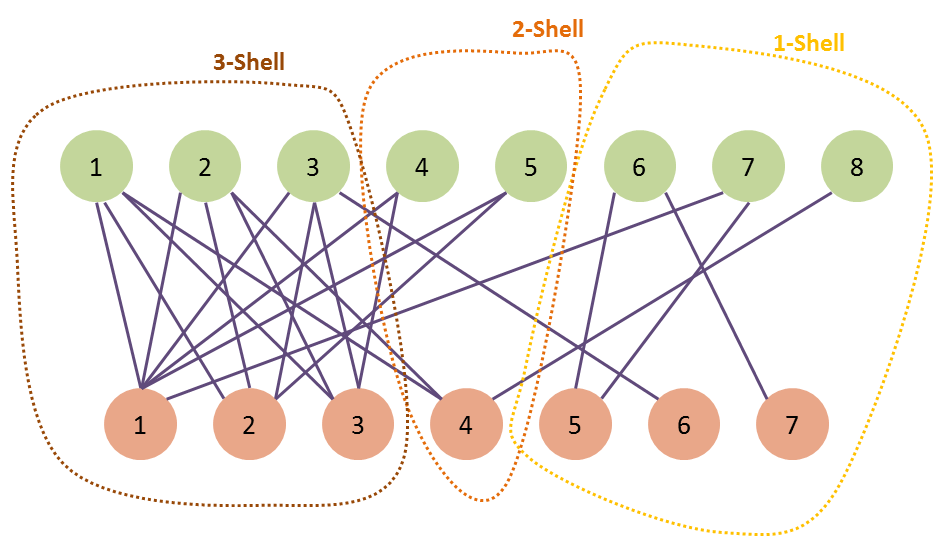
\includegraphics[scale=0.5]{Figures/ESTATICA_kcore_decomposition_example.png}
\caption{Descomposición \textit{k-core} de una red bipartita ficticia.}
\label{fig:ESTATICA_kcore_decomposition_example}
\end{figure}

Según la definición \ref{ESTATICA_def_kcore}, el  \textit{1-core} es la unión de las tres \textit{shell}, mientras que el \textit{2-core} es la unión de la \textit{2-shell} y la \textit{1-shell}. El \textit{k-core} máximo coincide con la  \textit{k-shell} máxima. 

Como estamos tratando de redes bipartitas, distinguimos dos subconjuntos en cada \textit{k-shell}, el de los nodos de la clase $A$ y el de los de la clase $B$. Los llamaremos $K^{A}_{j}, K^{B}_{j}$, donde  $j$ es el índice de la \textit{k-shell}.
Es posible que uno de ellos sea vacío, es decir, no todas las \textit{k-shell} tienen nodos de ambas clases necesariamente.
Al valor máximo de \textit{k}, lo llamamos $ks_{max}$, que corresponde a \textit{shell} más interna de la red $ks_{max}\equiv C^{A,B}$. Esta nomenclatura simplifica la definición de las \textit{k-magnitudes} que surgen de la red descompuesta siguiendo el procedimiento descrito.


\section{K magnitudes}

Las especies más conectadas de una red mutualista son resistentes a las perturbaciones externas porque el beneficio que reciben depende de múltiples fuentes. Esta parece ser la razón por la que las redes mutualistas tienden al anidamiento, una conexión directa con el centro de la red aumenta las probabilidades de supervivencia. Para medir la 'distancia' desde un nodo cualquiera a la \textit{k-shell} más interna de la clase opuesta, hemos definido el \textit{$k_{radius}$}.

\begin{theo} 
El \textit{$k_{radius}$} del nodo $m$ de la clase $A$ es el valor medio de la distancia a las especies de $C^B$
\begin{align*}
\displaystyle
k^A_{radius}m = \frac{1}{\mid C^{B} \mid}\sum\limits_{j \in C^{B}} dist_{mj}  \qquad   m \in A
\stepcounter{equation}\tag{\theequation}\label{kradius}
\end{align*}
\label{ESTATICA_kradius}
\end{theo}

En la fórmula \ref{ESTATICA_kradius} $dist_{mj}$ es el camino más corto de la especie $m$ a cada una de las $j$ especies que forman el conjuto $C^B$. La misma definción es válida para especies de la clase $B$, calculando la distancia media a las especies de $C^A$. El valor mínimo posible de $k_{radius}$ es $1$ para un nodo perteciente a $C^B$ conectado con todas las especies de $C^A$ (y viceversa).

\begin{figure}[h!]
\centering
\includegraphics[scale=0.58]{ESTATICA_red_example.eps}
\caption {Cálculo de \textit{$k_{radius}$} y  \textit{$k_{degree}$} en una red ficticia.}
\label{fig:ESTATICA_red_example}
\end{figure}

La parte superior izquierda de la figura \ref{fig:ESTATICA_red_example} es el esquema de otra red ficticia muy sencilla, con solo siete nodos, tres de la clase $A$ y cuatro de la $B$. Como se puede ver,  la especie $B4$ es la única que pertenece a la $1$-$shell$. El resto son parte de las $2$-$shell$, que por ser la más internas se toman como referencia para medir los $k_{radius}$ individuales. 

En la parte superior derecha de la imagen, se reproduce el detalle de las conexiones de la especie $A1$, perteneciente a $C^{A}$.  Como está directamente conectada con los tres nodos de $C^{B}$ la el camino más corto a cada uno de ellos es $1$, y en consecuencia $k^A_{radius}1$ es $1$. En la parte inferior derecha, la especie $A2$ que también pertenece a $C^{A}$ no tiene enlace directo con $B2$, aunque sí con $B1$ y $B3$. El camino más corto, marcado en color violeta, pasa por $B1$ y $A1$, y mide $3$. El $k^A_{radius}2$ vale $\sfrac{5}{3}$. En la parte inferior izquierda, vemos el esquema de conexiones de la especie $B4$, que no forma parte de $C^{B}$. Como cabía esperar, su$k_{radius}$ es mayor, $\sfrac{7}{3}$. 

Podemos definir una magnitud global, teniendo en cuenta los $k_{radius}$ de todas las especies.

\begin{theo} 
El \textit{$\overline k_{radius}$} de una red se obtiene promediando los ${k}_{radius}$ de todos los nodos, sin importar la clase a la que pertenezcan.
\begin{align*}
\displaystyle
\overline {k}_{radius} = \frac{1}{\mid A \cup B \mid}\sum\limits_{l \in A \cup B} k_{radius}l
\stepcounter{equation}\tag{\theequation}\label{avgkradius}
\end{align*}
\label{ESTATICA_avgkradius}
\end{theo}

Una red con todos sus nodos conectados (matriz de adyacencia cuadrada) tendría $\overline {k}_{radius}=1$, el menor posible. En una con matriz de adyacencia triangular el $\overline {k}_{radius}$ vale $1.5$. En la red que hemos usado como ejemplo, su valor es $\sfrac{11}{7}$. Intuitivamente, el $\overline {k}_{radius}$ será pequeño para redes muy anidadas, porque la probabilidad de conexión con la \textit{shell} más interna es elevada. Las especies generalistas están muy interconectadas y las especialistas tienen enlaces directos con las \textit{k-shells} de mayor índice. por el contrario, una distribución de enlaces puramente aleatoria conduciría a una red con mayor $\overline {k}_{radius}$.

El ${k}_{radius}$ es una buena medida de conexión al corazón de la red pero no de centralidad. Por ejemplo, su valor es bajo para un especialista con un enlace a la \textit{shell} más interna, aunque sabemos que no resulta determinante para la estabilidad global de la red. Para atender esta necesidad, definimos una segunda \textit{k-magnitud}.

\begin{theo} 
\begin{align*}
\displaystyle
k^A_{degree}m = \sum\limits_{j} \frac{a_{mj} }{k_{radius}j}  \quad   m \in A, \forall j \in B
\stepcounter{equation}\tag{\theequation}
\end{align*}
\label{kdegree}
\end{theo}

Donde $a_{mj}$ es el elemento de la matriz de interacción que representa el enlace, cuyo valor es $1$ si existe o $0$ si no está presente. El $k_{degree}$ es la suma de los inversos de los $k_{radius}$ de los nodos conectados con $m$. Una especie de la \textit{shell} más interna tiene un $k_{degree}m$ elevado,  mientras que los especialistas con solo uno o dos enlaces tiene un $k_{degree}$ reducido. Volviendo al ejemplo de la figura \ref{fig:ESTATICA_red_example}, el $k_{degree}$ del nodo $B3$ es is $1+\sfrac{3}{5}+\sfrac{3}{5} = \sfrac{11}{5}$, mientras que solo vale $\sfrac{3}{7}$ para el especialista $B4$. Esta magnitud recuerda la definición del \textit{índice de Harary} \cite{plavvsic1993harary} pero teniendo solo en cuenta los enlaces con la \textit{shell} más interna.


\subsection{Algoritmo de destrucción basado en \textit{k-shell}}

Para poder establecer políticas de conservación es necesario disponer de un respaldo cuantitativo, localizando a las especies que más contribuyen a la estabilidad de las redes \cite{sole2001fragility, dakos2015resilience, thebault2010stability, suweis2013emergence, santamaria2015removing}.  Hay dos aproximaciones posibles. La primera se basa en la dinámica de ponlaciones y depende en gran medida de la parametrización del modelo elegido \cite{dakos2014critical}. La segunda, que utiliza solo la topología de la red, es más sencilla de implementar y por tanto mucho más popular. Es la que seguimos en este capítulo.

La biodiversidad y resistencia de una comunidad mutualista depende de su estructura. La extinción de algunas especies provoca que partes de la red queden desconectadas de la componente gigante y posiblemente expuestas a la desaparición. Por este motivo, la evolución del tamaño de la componente gigante cuando se eliminan especies es el criterio más utilizado para estudiar la resistencia estructural estática.

Esto es lo que hace el método de medida de Dunne \cite{dunne2002biodiversity}, ideado en origen para \textit{food webs}. Las especies se van retirando una por una de la red (extinciones primarias). Este hecho produce extinciones secundarias de aquellas especies. La gráfica de la fracción de la red inicial superviviente, frente a la fracción de extinciones primarias (en escala normalizada entre 0 y 1) define la \textit{curva de extinción}. Cuanto menor sea el área bajo esta curva, más rápida será la destrucción de la red.

\begin{figure}[h!]
\centering
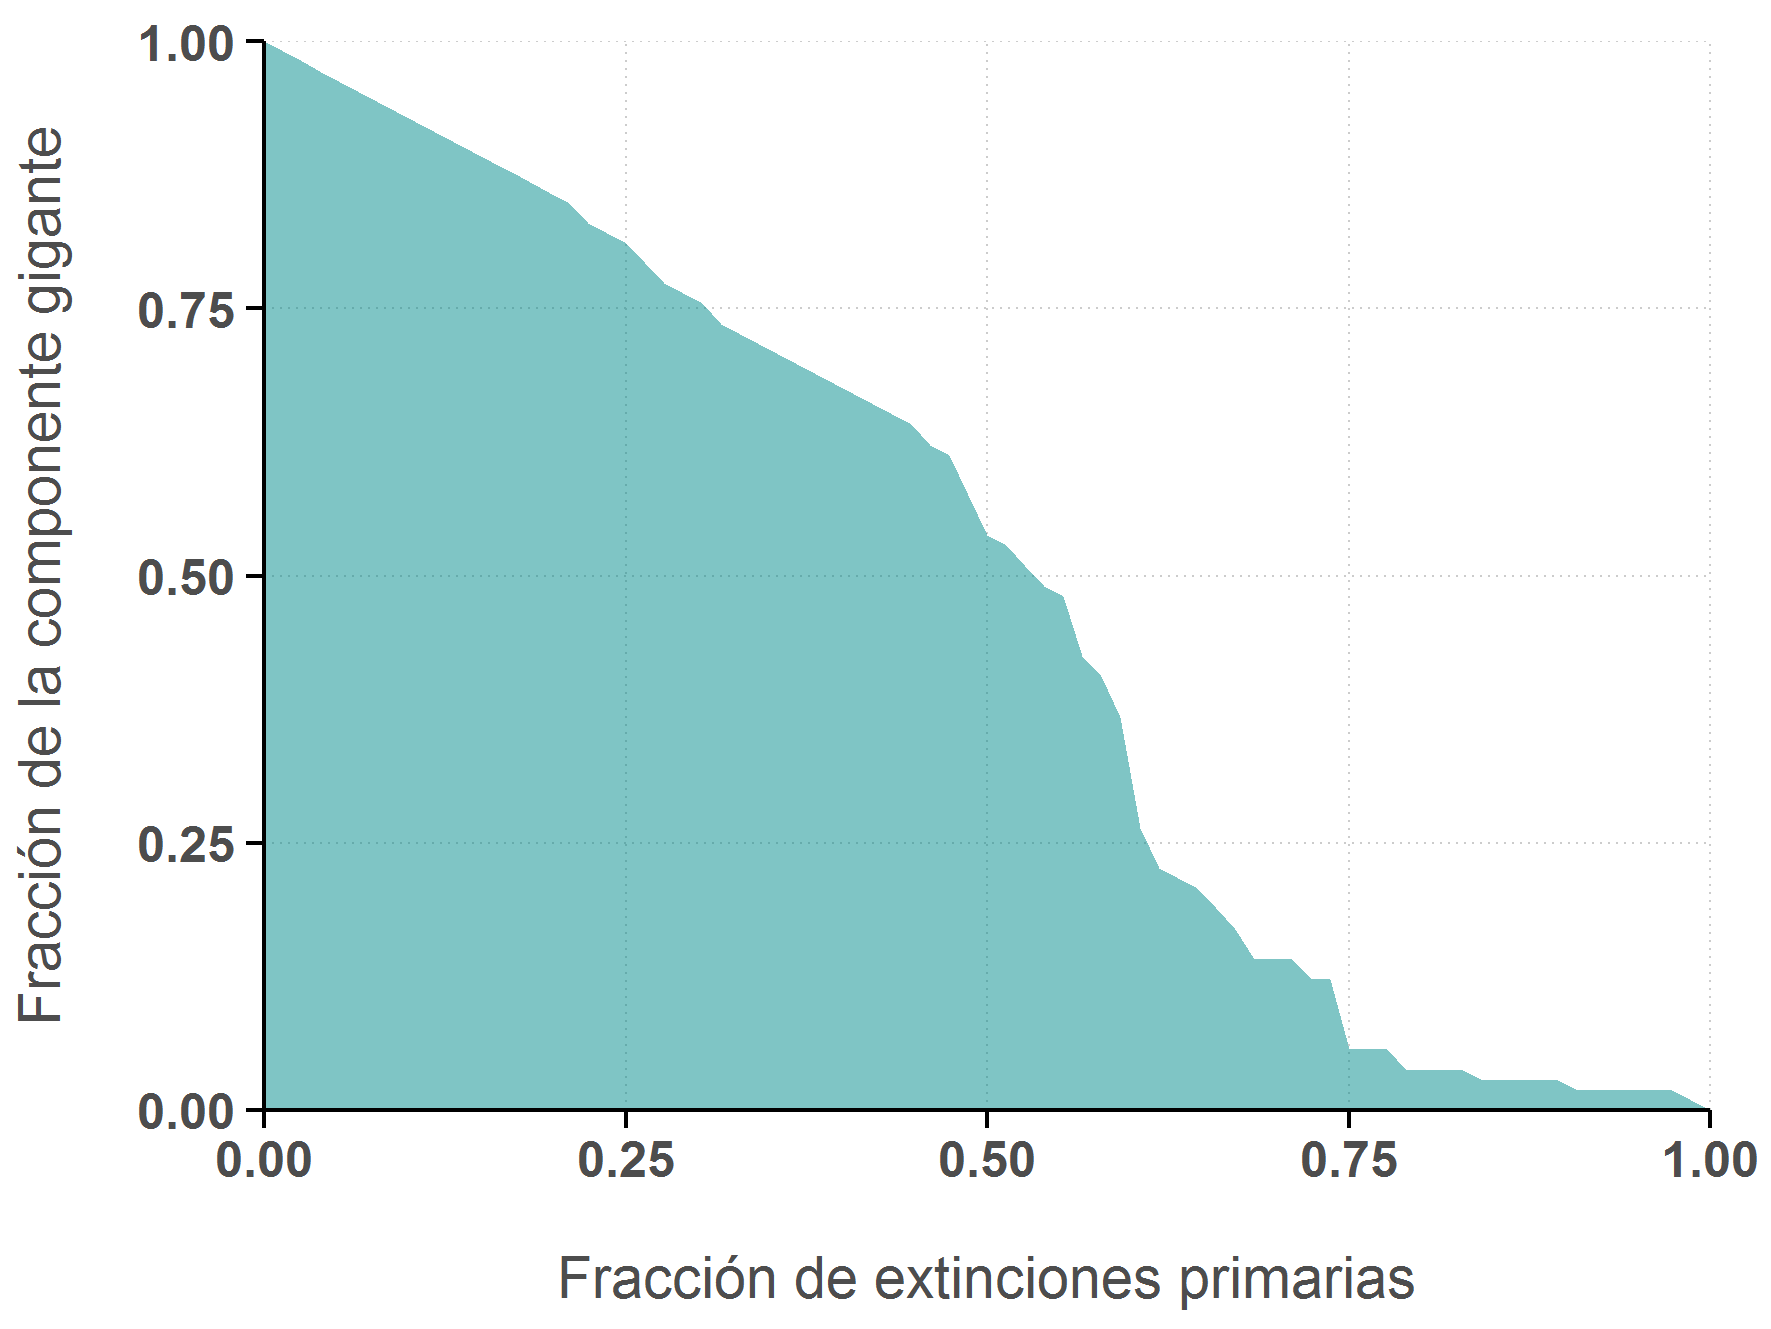
\includegraphics[scale=0.55]{Figures/ESTATICA_destruction_example.png}
\caption{Ejemplo de curva de extinción siguiendo el método de Dunne. El área bajo la curva indica la velocidad a la que se desintegra la componente gigante.}
\label{fig:ESTATICA_destruction_example}
\end{figure}

La clave está en el orden de selección de las especies que se retiran en las extinciones primarias. Si disponemos de una cifra que defina su importancia para esa red concreta, se podrán concentrar los esfuerzos de conservación en las especies que más aportan a la supervivencia del sistema. El problema es que no existe un criterio universalmente aceptado para establecer esa clasificación que resulte óptimo para cualquier red.

En el mutualismo, parece lógico pensar que las especies de las \textit{shells} más internas son las más importantes para mantener la integridad de la red. El algoritmo de destrucción que proponemos se basa en la secuencia $k$-$shell, k_{degree}, k_{radius}$, esto es, se empiezan las extinciones primarias por las especies pertenecientes a la $k$-$shell$ de mayor índice, y dentro de esta, el de mayor $k_{degree}$, y en caso de coincidencia, el de menor $k_{radius}$. 

\section{Material y métodos}

Para este capítulo hemos utilizado la colección de datos de redes mutualistas de la \textit{Web of Life}  \url{http://www.web-of-life.es/} \cite{fortuna2014web}. Hemos analizado todas las disponibles en las categorías \textit{planta-polinizador} y \textit{planta-dispersor de semillas}. En diciembre de 2015 dicha colección consta de 59 redes de la primera familia y 30 de la segunda. El número de especies por red varía entre 6 y 997 y el número de interacciones entre 6 y 2993.

El software se ha desarrollado en \texttt{R} y \texttt{Python}. La \textit{descomposición k-core} se realiza con el paquete \texttt{R} \texttt{igraph} \cite{csardi2006igraph}. El mismo paquete ofrece funciones para el cálculo de $NODF$ y $Modularity$. El código \texttt{R} para medir ${k}_{degree}$ y ${k}_{radius}$ es propio. Los valores medios de estas magnitudes se calculan descartando las especies que no pertenecen a la componente gigante cuando en la red se produce esta circunstancia. 

Para medir la bondad del algoritmo de destrucción, hemos comparado su rendimiento con el que ofrece \textit{MusRank}, de reciente publicación y basado en una clasificación de la importancia de los nodos similar a la del \textit{PageRank} de Google  \citep{dominguez2015ranking}. Tanto el algoritmo basado en \textit{k-shell} como la medición del \textit{MusRank} se han codificado en \texttt{Python}.

\begin{table}[htbp]
\tiny
  \centering
    \begin{tabular}{lrrrrrrrrr}
    \toprule
    $Red$  & $Plantas$ & $Animales$ & $Enlaces$ & $k_{max}$ & $\overline k_{degree}$ & $\overline k_{radius}$ & $NODF$ & $Modularity$ & $Area_{Mus-k}$ \\
    \midrule
 
    M\_PL\_001 & 84   & 101  & 361  & 4    & 1,56 & 3,01 & 14,46 & 0,45 & 0,08 \\
    M\_PL\_002 & 43   & 64   & 196  & 3    & 1,4  & 3,04 & 15,36 & 0,48 & 0,11 \\
    M\_PL\_003 & 36   & 25   & 81   & 2    & 0,93 & 3,31 & 19,19 & 0,57 & 0,02 \\
    M\_PL\_004 & 12   & 102  & 167  & 3    & 1,52 & 2,53 & 28,15 & 0,45 & 0,09 \\
    M\_PL\_005 & 96   & 275  & 923  & 8    & 2,54 & 2,8  & 14,74 & 0,24 & 0,14 \\
    M\_PL\_006 & 17   & 61   & 146  & 4    & 2,28 & 2,44 & 44,58 & 0,33 & 0,04 \\
    M\_PL\_007 & 16   & 36   & 85   & 3    & 1,68 & 2,51 & 31,54 & 0,36 & 0,12 \\
    M\_PL\_008 & 11   & 38   & 106  & 4    & 2,19 & 2,37 & 35,97 & 0,21 & 0,03 \\
    M\_PL\_009 & 24   & 118  & 242  & 4    & 1,54 & 2,81 & 15,39 & 0,44 & 0,16 \\
    M\_PL\_010 & 31   & 76   & 456  & 8    & 4,57 & 2,38 & 35,17 & 0,02 & 0,03 \\
    M\_PL\_011 & 14   & 13   & 52   & 3    & 2,27 & 2,16 & 54,59 & 0,29 & 0 \\
    M\_PL\_012 & 29   & 55   & 145  & 4    & 2,01 & 2,51 & 30,4 & 0,42 & 0,05 \\
    M\_PL\_013 & 9    & 56   & 103  & 4    & 1,96 & 2,4  & 34,25 & 0,38 & 0,14 \\
    M\_PL\_014 & 29   & 81   & 179  & 3    & 1,48 & 2,8  & 25,68 & 0,44 & 0,08 \\
    M\_PL\_015 & 131  & 666  & 2933 & 9    & 2,9  & 2,88 & 9,17 & 0,35 & 0,08 \\
    M\_PL\_016 & 26   & 179  & 412  & 5    & 1,88 & 2,73 & 21,98 & 0,42 & 0,15 \\
    M\_PL\_017 & 25   & 79   & 299  & 6    & 3,28 & 2,47 & 40,37 & 0,15 & 0,04 \\
    M\_PL\_018 & 39   & 105  & 383  & 5    & 2,26 & 2,74 & 19,73 & 0,24 & 0,11 \\
    M\_PL\_019 & 40   & 85   & 264  & 5    & 1,97 & 2,71 & 17,51 & 0,34 & 0,13 \\
    M\_PL\_020 & 20   & 91   & 190  & 4    & 1,84 & 2,56 & 37,12 & 0,39 & 0,09 \\
    M\_PL\_021 & 91   & 677  & 1193 & 5    & 1,23 & 3,06 & 7,55 & 0,58 & 0,21 \\
    M\_PL\_022 & 21   & 45   & 83   & 2    & 0,84 & 3,68 & 18,02 & 0,6  & 0,14 \\
    M\_PL\_023 & 23   & 72   & 125  & 3    & 1,35 & 2,75 & 22,88 & 0,54 & 0,14 \\
    M\_PL\_024 & 11   & 18   & 38   & 3    & 1,71 & 1,97 & 29,02 & 0,42 & 0,16 \\
    M\_PL\_025 & 13   & 44   & 143  & 5    & 3,4  & 2,13 & 46,02 & 0,16 & 0 \\
    M\_PL\_026 & 105  & 54   & 204  & 3    & 1,13 & 2,85 & 25,13 & 0,56 & 0,11 \\
    M\_PL\_027 & 18   & 60   & 120  & 3    & 1,2  & 2,96 & 13,94 & 0,55 & 0,19 \\
    M\_PL\_028 & 41   & 139  & 374  & 5    & 2,11 & 2,75 & 16,43 & 0,37 & 0,1 \\
    M\_PL\_029 & 49   & 118  & 346  & 5    & 1,94 & 2,76 & 15,77 & 0,41 & 0,12 \\
    M\_PL\_030 & 28   & 53   & 109  & 2    & 0,83 & 3,54 & 11,16 & 0,54 & 0,17 \\
    M\_PL\_031 & 48   & 49   & 156  & 4    & 1,57 & 3,39 & 12,34 & 0,54 & 0,05 \\
    M\_PL\_032 & 7    & 33   & 65   & 3    & 2,41 & 2,07 & 56,66 & 0,1  & 0,05 \\
    M\_PL\_033 & 13   & 34   & 141  & 5    & 3,4  & 2,24 & 29,5 & 0,07 & 0,04 \\
    M\_PL\_034 & 26   & 128  & 312  & 5    & 2,1  & 2,61 & 25,01 & 0,42 & 0,08 \\
    M\_PL\_035 & 61   & 36   & 178  & 4    & 1,74 & 2,85 & 25,74 & 0,43 & 0 \\
    M\_PL\_036 & 10   & 12   & 30   & 2    & 1,31 & 2,51 & 35,96 & 0,38 & 0,09 \\
    M\_PL\_037 & 10   & 40   & 72   & 3    & 1,37 & 2,7  & 23,16 & 0,44 & 0,14 \\
    M\_PL\_038 & 8    & 42   & 79   & 3    & 1,56 & 2,44 & 28,31 & 0,39 & 0,06 \\
    M\_PL\_039 & 17   & 51   & 129  & 4    & 1,99 & 2,61 & 25,34 & 0,45 & 0,12 \\
    M\_PL\_040 & 29   & 43   & 114  & 3    & 1,32 & 2,92 & 15,18 & 0,5  & 0,03 \\
    M\_PL\_041 & 31   & 43   & 145  & 4    & 2,11 & 2,51 & 25,3 & 0,35 & 0,11 \\
    M\_PL\_042 & 12   & 6    & 25   & 3    & 2,34 & 1,71 & 49,79 & 0,33 & 0,07 \\
    M\_PL\_043 & 28   & 82   & 250  & 4    & 1,99 & 2,71 & 22,17 & 0,29 & 0,1 \\
    M\_PL\_044 & 110  & 609  & 1125 & 4    & 1,12 & 3,36 & 4,92 & 0,57 & 0,22 \\
    M\_PL\_045 & 17   & 26   & 63   & 3    & 1,73 & 2,43 & 30,77 & 0,45 & 0,09 \\
    M\_PL\_046 & 16   & 44   & 278  & 8    & 6,45 & 1,96 & 63,6 & -0,03 & 0 \\
    M\_PL\_047 & 19   & 186  & 425  & 6    & 2,31 & 2,56 & 29,96 & 0,29 & 0,09 \\
    M\_PL\_048 & 30   & 236  & 671  & 7    & 2,78 & 2,61 & 26,23 & 0,21 & 0,08 \\
    M\_PL\_049 & 37   & 225  & 590  & 6    & 2,08 & 2,76 & 18,13 & 0,38 & 0,14 \\
    M\_PL\_050 & 14   & 35   & 86   & 3    & 1,71 & 2,49 & 32,58 & 0,43 & 0,08 \\
    M\_PL\_051 & 14   & 90   & 164  & 4    & 2,13 & 2,34 & 26,96 & 0,45 & 0,1 \\
    M\_PL\_052 & 15   & 39   & 92   & 3    & 1,7  & 2,51 & 30,91 & 0,31 & 0,14 \\
    M\_PL\_053 & 99   & 294  & 589  & 3    & 0,92 & 3,8  & 4,71 & 0,58 & 0,2 \\
    M\_PL\_054 & 113  & 318  & 773  & 5    & 1,42 & 3,07 & 8,08 & 0,46 & 0,2 \\
    M\_PL\_055 & 64   & 195  & 431  & 4    & 1,29 & 3,13 & 8,71 & 0,52 & 0,19 \\
    M\_PL\_056 & 91   & 365  & 871  & 5    & 1,43 & 3,24 & 6,86 & 0,46 & 0,17 \\
    M\_PL\_057 & 114  & 883  & 1920 & 8    & 1,8  & 2,88 & 7,04 & 0,48 & 0,23 \\
    M\_PL\_058 & 32   & 81   & 319  & 6    & 3,03 & 2,48 & 26,64 & 0,22 & 0,06 \\
    M\_PL\_059 & 13   & 13   & 71   & 5    & 4,72 & 1,57 & 76,88 & 0,04 & 0,01 \\
    M\_SD\_001 & 7    & 21   & 50   & 3    & 2,33 & 2,16 & 40,77 & 0,18 & 0,06 \\
    M\_SD\_002 & 31   & 9    & 119  & 6    & 4,61 & 1,85 & 62,16 & 0,02 & -0,02 \\
    M\_SD\_003 & 25   & 16   & 68   & 3    & 1,78 & 2,45 & 41,09 & 0,33 & 0,05 \\
    M\_SD\_004 & 34   & 20   & 95   & 4    & 2,37 & 2,19 & 39,82 & 0,35 & 0,01 \\
    M\_SD\_005 & 25   & 13   & 49   & 3    & 1,33 & 2,38 & 27,93 & 0,53 & 0,1 \\
    M\_SD\_006 & 21   & 15   & 51   & 3    & 1,51 & 2,35 & 32,79 & 0,45 & 0,08 \\
    M\_SD\_007 & 72   & 7    & 143  & 3    & 2,34 & 2,37 & 51,67 & 0,28 & 0 \\
    M\_SD\_008 & 16   & 10   & 110  & 7    & 6,56 & 1,48 & 56,33 & -0,04 & -0,01 \\
    M\_SD\_009 & 7    & 18   & 38   & 3    & 1,9  & 2,15 & 33,02 & 0,32 & 0,06 \\
    M\_SD\_010 & 50   & 14   & 234  & 6    & 4,48 & 2,14 & 42,13 & 0,04 & -0,1 \\
    M\_SD\_011 & 11   & 14   & 47   & 3    & 2,14 & 2,17 & 45,41 & 0,31 & 0,03 \\
    M\_SD\_012 & 35   & 29   & 146  & 4    & 2,31 & 2,57 & 33,04 & 0,23 & 0 \\
    M\_SD\_013 & 36   & 19   & 197  & 7    & 4,38 & 2,31 & 37,37 & 0,33 & -0,13 \\
    M\_SD\_014 & 16   & 17   & 121  & 5    & 5,16 & 1,87 & 78,76 & 0,08 & -0,01 \\
    M\_SD\_015 & 5    & 27   & 86   & 4    & 4,25 & 1,65 & 67,34 & 0,03 & -0,01 \\
    M\_SD\_016 & 24   & 61   & 500  & 11   & 8,4  & 2,01 & 58,84 & 0    & 0,01 \\
    M\_SD\_017 & 16   & 8    & 72   & 5    & 4,74 & 1,63 & 60,12 & 0,08 & -0,04 \\
    M\_SD\_018 & 29   & 32   & 66   & 2    & 0,75 & 3,41 & 11,21 & 0,59 & 0,21 \\
    M\_SD\_019 & 169  & 40   & 666  & 7    & 3,23 & 2,62 & 32,87 & 0,33 & -0,09 \\
    M\_SD\_020 & 25   & 33   & 150  & 5    & 3,07 & 2,31 & 53,55 & 0,13 & -0,01 \\
    M\_SD\_021 & 18   & 28   & 129  & 5    & 3,46 & 2,19 & 61,52 & 0,18 & -0,01 \\
    M\_SD\_022 & 207  & 110  & 1121 & 8    & 3,21 & 2,8  & 16,81 & 0,2  & -0,01 \\
    M\_SD\_023 & 15   & 8    & 38   & 3    & 2,3  & 2,03 & 66,8 & 0,22 & 0 \\
    M\_SD\_024 & 12   & 7    & 40   & 3    & 2,5  & 1,99 & 56,83 & 0,12 & -0,02 \\
    M\_SD\_025 & 7    & 6    & 22   & 3    & 2,41 & 1,69 & 66,67 & 0,19 & 0 \\
    M\_SD\_026 & 3    & 3    & 6    & 2    & 1,83 & 1,33 & 100  & 0,17 & 0 \\
    M\_SD\_027 & 12   & 4    & 31   & 4    & 3,45 & 1,53 & 73,61 & 0    & 0 \\
    M\_SD\_028 & 8    & 5    & 26   & 4    & 3,65 & 1,38 & 89,47 & 0,02 & 0 \\
    M\_SD\_029 & 4    & 5    & 10   & 2    & 1,98 & 1,52 & 81,25 & 0,27 & 0 \\
    M\_SD\_030 & 5    & 4    & 11   & 2    & 2,24 & 1,5  & 66,67 & 0,23 & 0 \\
    
    \bottomrule
    \end{tabular}%
    \caption{\label{table:table_results} Propiedades de las redes utilizadas en el estudio.}

\end{table}%

\section{Resultados}

En este apartado se describen los resultados de los siguientes procedimientos: análisis exploratorio de los datos de las redes de la colección, estudio de la correlación entre las \textit{k-magnitudes} las medidas estadísticas habituales, experimento de recableado y comparación del algoritmo de destrucción basado en \textit{k-shell} con el basado en \textit{MusRank}.

\subsection{Análisis exploratorio}

En la figura \ref{fig:ESTATICA_hist_kmagnitudes} se han representado los histogramas de las tres \textit{k-magnitudes} que describen globalmente las redes incluidas en la investigación. En la mitad de ellas el índice $k$ máximo es $4$ o menos y solo hay dos que tengan más de $8$. La distribución del $\overline{k}_{radius}$ es aproximadamente normal, con una mediana de $2,51$ y media $2,47$. Teniendo en cuenta que el valor mínimo de esta magnitud es $1$, podemos deducir que las redes mutualistas analizadas son \textit{very small world}, las especies se encuentran muy próximas a la \textit{k-shell} más interna. Este dato concuerda con la observación de que los especialistas se conectan con generalistas lo que les proporciona más probabilidades de supervivencia. Finalmente, el $\overline{k}_{degree}$ se
concentra entre los valores $0,5$ y $3,5$ con la mediana en $2,08$. La conectividad media de las redes es reducida
porque abundan los especialistas. En el tercer histograma hay una diferencia sensible entre las redes de polinizadores
y las de dispersores de semillas, pues estas últimas tienen valores más elevados.

\begin{figure}[h!]
\centering
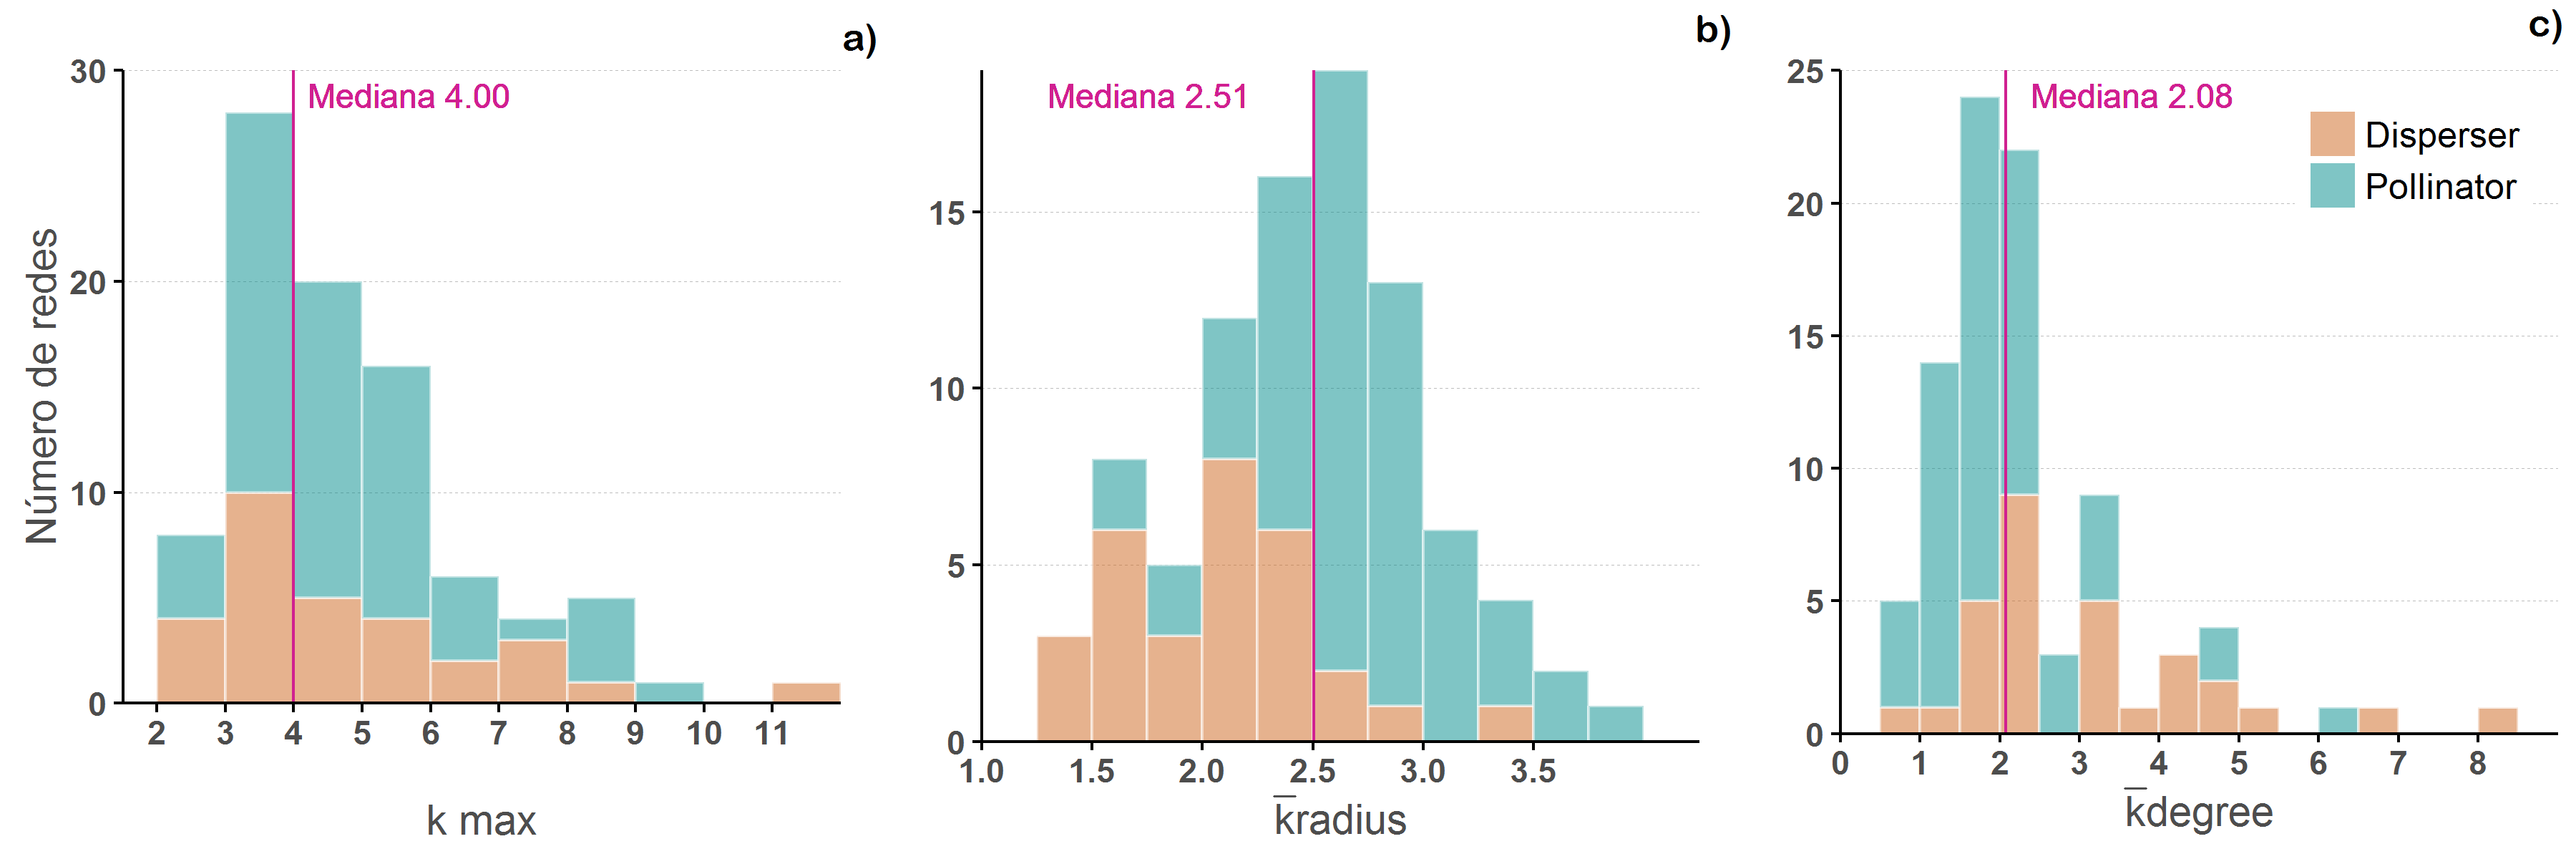
\includegraphics[scale=0.5]{Figures/ESTATICA_hist_kmagnitudes.png}
\caption{Histogramas de las \textit{k-magnitudes}.}
\label{fig:ESTATICA_hist_kmagnitudes}
\end{figure}

En una primera aproximación visual a los datos, encontramos que existía una alta correlación entre el $\overline{k}_{radius}$ de la red y el número de especies (figura \ref{fig:ESTATICA_tamanyo_kdegree_kradius}). Como cabía esperar, cuanto mayor es la red, mayor es la distancia media a la \textit{shell} máxima. El crecimiento sigue una ley logarítmica, nótese la escala del eje $X$. Sucede algo parecido con el número de enlaces, pero en este caso se puede apreciar mayor dispersión. 

Por el contrario, el $\overline{k}_{degree}$ no parece guardar ninguna relación con el tamaño de la red, ya se mida en número total de especies o de enlaces. Vemos que para la mayoría de redes su valor está en torno a $2$. Este dato hace sospechar que la distribución del ${k}_{degree}$ en las redes sigue una exponencial decreciente. La mayoría de los nodos tienen valores bajos, por lo que la media arroja ese valor tan pequeño. En la figura \ref{fig:ESTATICA_density_plots} aparecen las gráficas de dicha distribución de tres redes en las que resulta evidente la asimetría. 

\begin{figure}[h!]
\centering
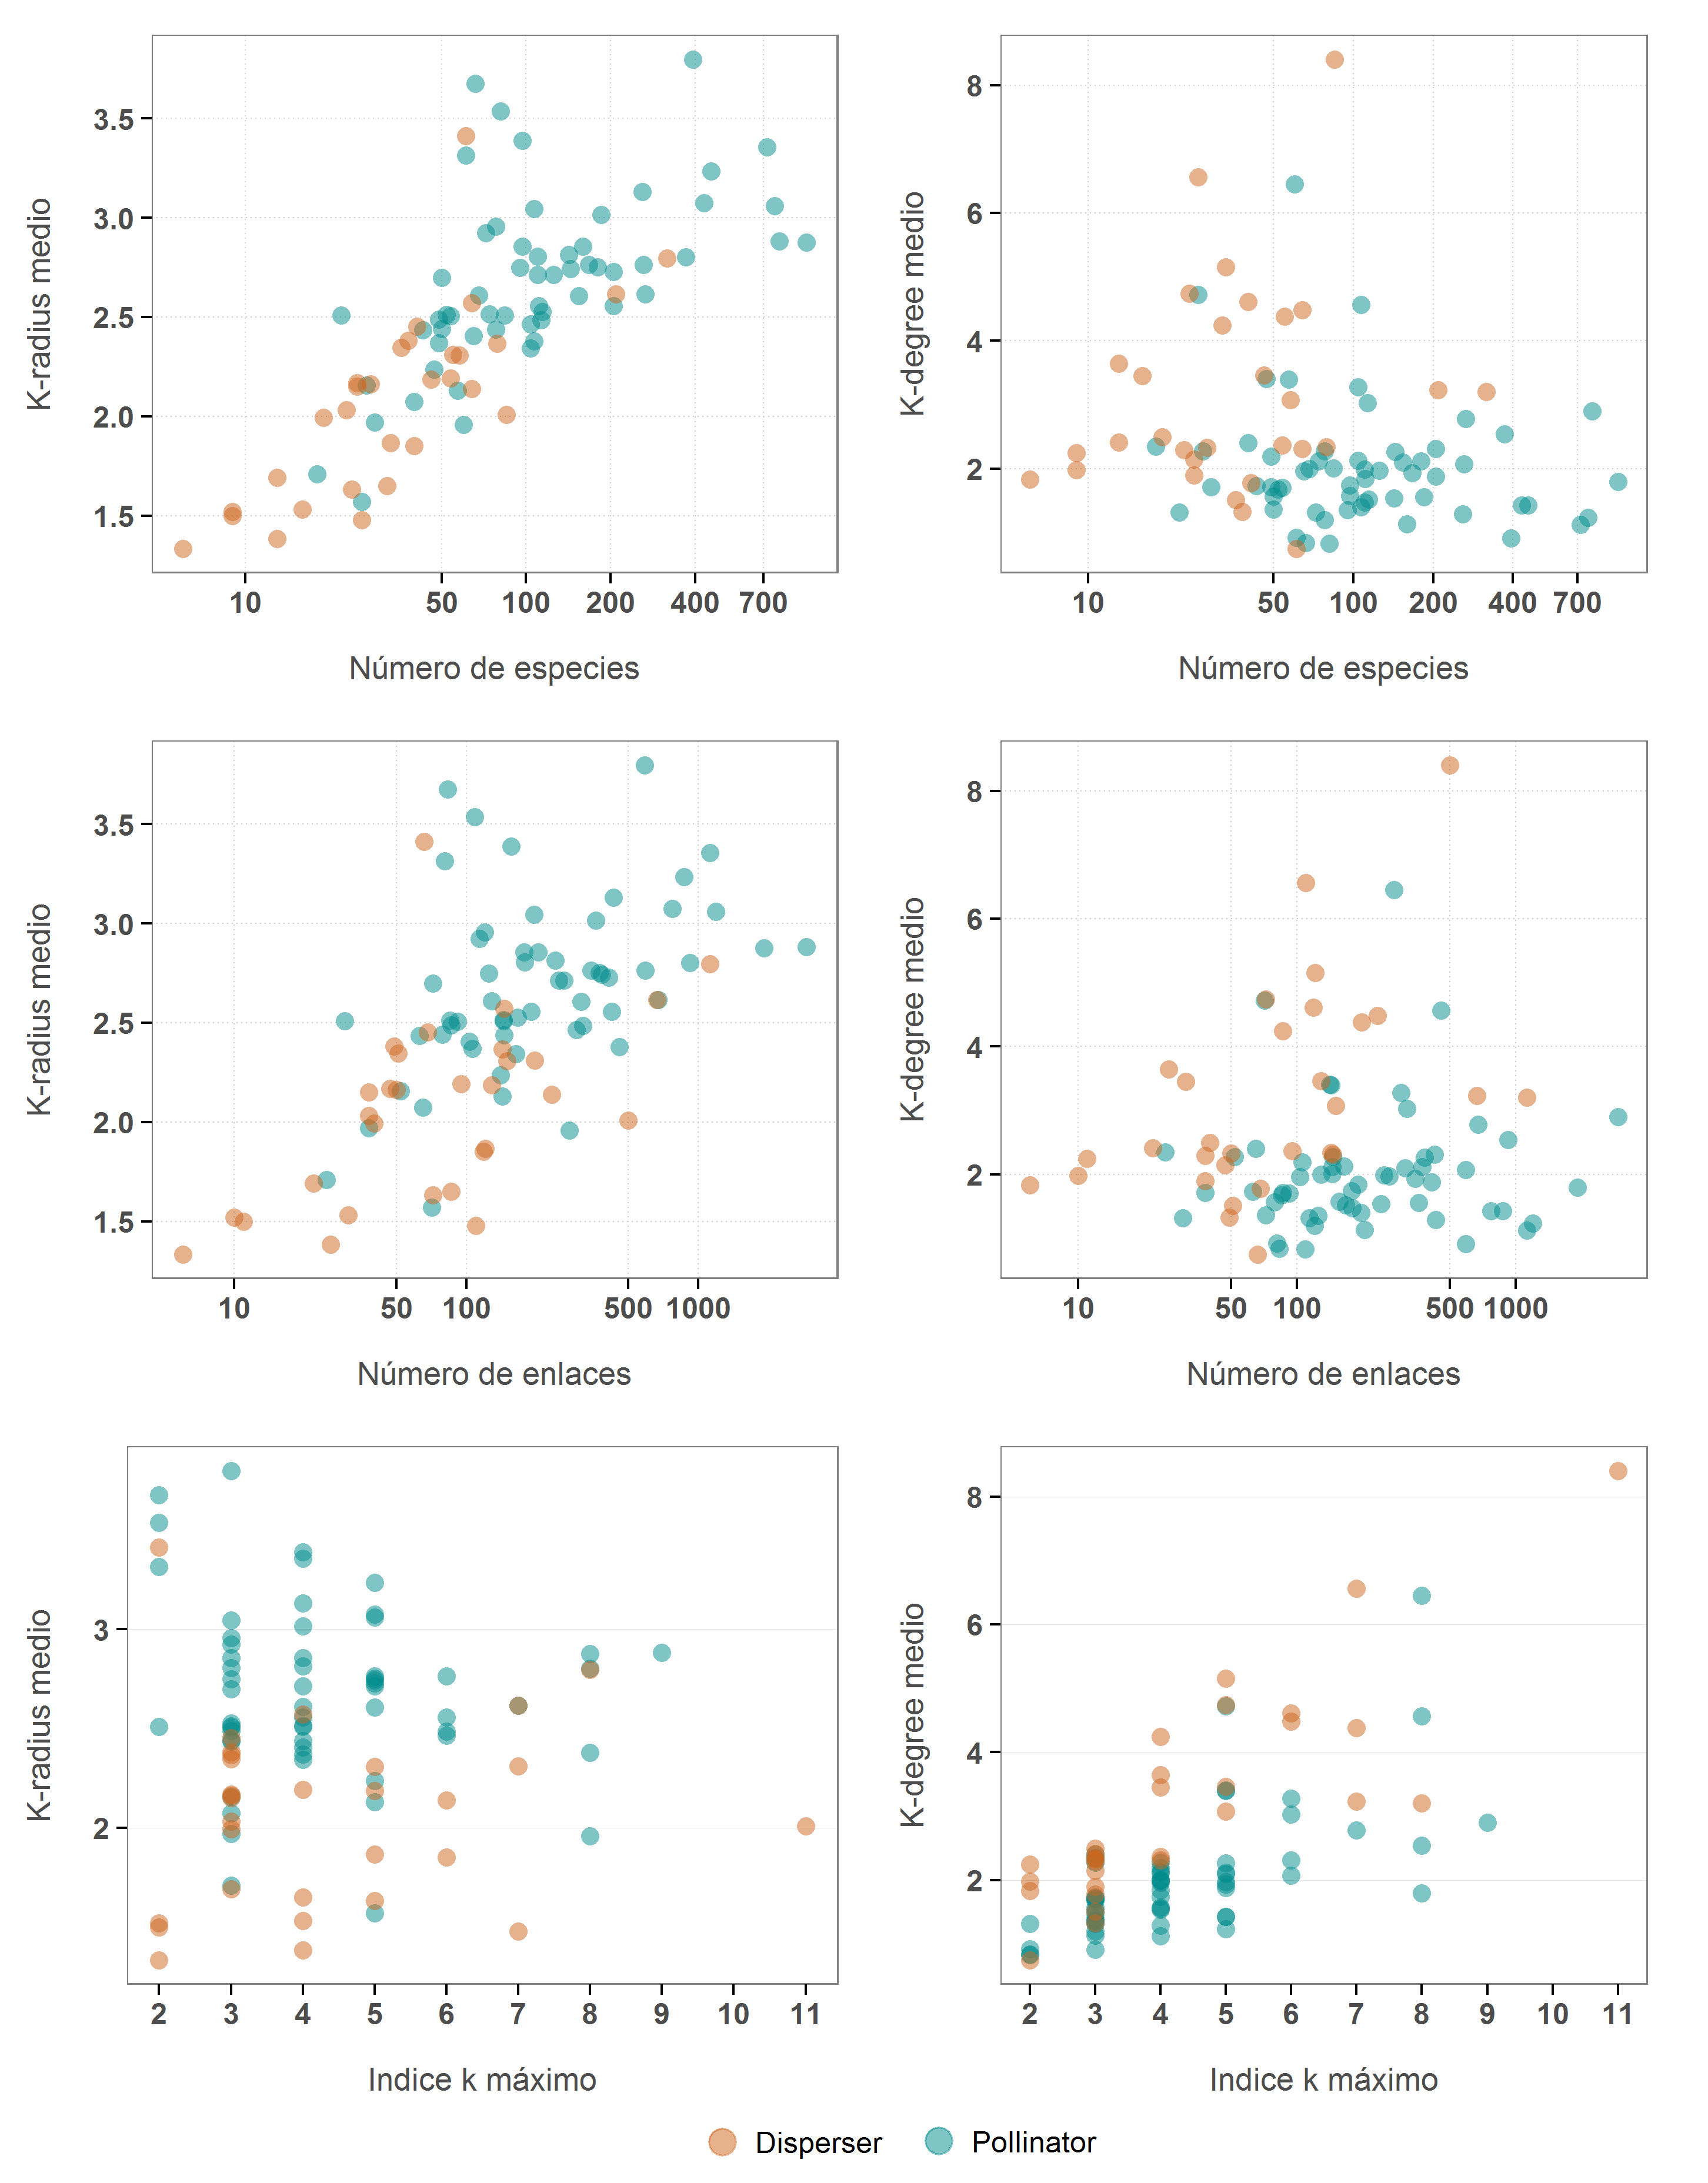
\includegraphics[scale=0.18]{Figures/ESTATICA_tamanyo_kdegree_kradius.png}
\caption{Diagramas de dispersión que relacionan las \textit{k-magnitudes} con el tamaño de la red.}
\label{fig:ESTATICA_tamanyo_kdegree_kradius}
\end{figure}

Si observamos la relación entre las dos \textit{k-magnitudes} y el indíce $k$ máximo de la red, descubrimos que la relación es inversa, el $\overline{k}_{degree}$ crece con el índice y el $\overline{k}_{radius}$ disminuye. No obstante, se aprecia una importante dispersión para redes con un mismo $k$ máximo.


\subsection{Correlación entre \textit{k-magnitudes} y propiedades globales}

Uno de los objetivos principales de la investigación es hallar la posible relación entre las magnitudes que se derivan de la \textit{descomposición k-core} y las que se utilizan habitualmente en la caracterización del mutualismo. Hemos encontrado que las \textit{k-magnitudes} globales tienen una fuerte correlación con estas dos medidas, y esto es de gran interés puesto que surgen de la agregación de las propiedades locales de cada nodo.

Para realizar la comparación se calcula el anidamiento mediante \textit{NODF} y la modularidad siguiendo la definición de \textit{Modularity} de Newman \cite{almeida2008consistent, newman2004finding} \footnote{Para evitar confusiones entre el nombre la de la magnitud y la medida según un algoritmo concreto, en lo sucesivo se emplea \textit{Modularity}, en inglés y con mayúscula, para referirse al valor definido por Newman.}. Ambas medidas las proporciona el paquete \texttt{bipartite} en \texttt{R}. En la figura \ref{fig:ESTATICA_corrfigs} se han representado el $\overline {k}_{radius}$ en función de $NODF$ y el $\overline {k}_{degree}$ en función de la $modularidad$. Las figuras sugerían que existe un fuerte correlación negativa entre el $\overline {k}_{radius}$ y $NODF$ por una parte y, por otra, entre el $\overline {k}_{degree}$ y la $modularidad$. 

\begin{figure}[h!]
\centering
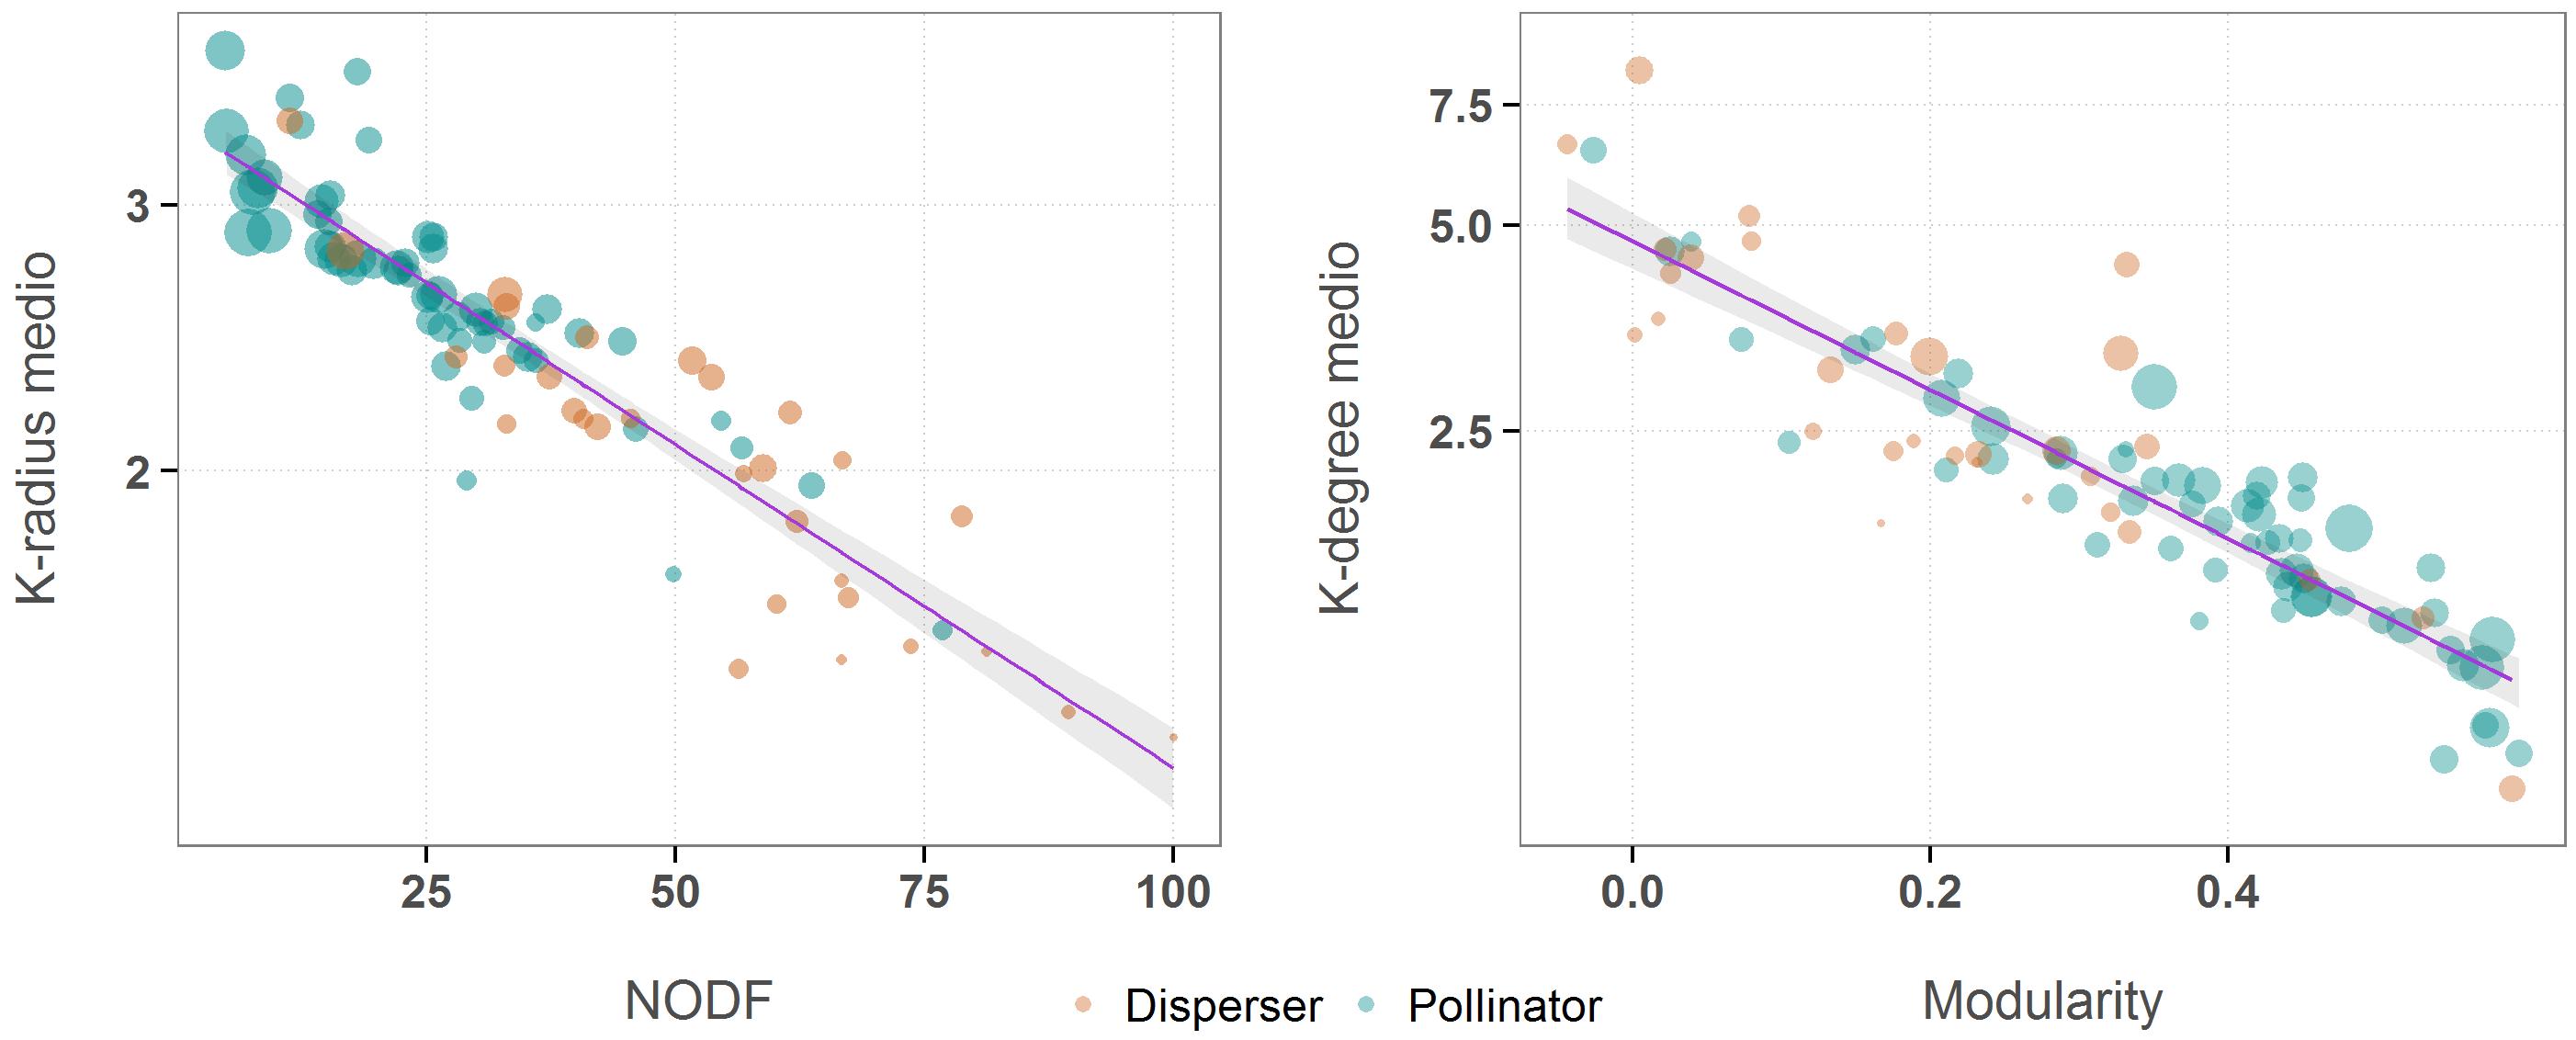
\includegraphics[scale=0.2]{ESTATICA_correlation_figs.png}
\caption {Diagrama de dispersión del $\overline {k}_{radius}$ respecto a $NODF$ (izquierda), y del $\overline {k}_{degree}$ respecto a la $Modularity$ (derecha). Cada punto es una red, su área es proporcional al logaritmo del número de especies y el color indica la clase de comunidad. Se han incluido las líneas de regresión con sus intervalos de confianza en sombreado.}
\label{fig:ESTATICA_corrfigs}
\end{figure}

Las nubes de puntos se representan sobre eje lineal en las abscisas y logarítmico en las ordenadas. Parecen compatibles con un modelo exponencial, así que procedimos a calcular las regresiones lineales $log(Y) ~ X$. Los resultados numéricos se resumen en la tabla \ref{table:table_lmodel}. Como muestra el valor ajustado de $R^2$ $(0,84)$, el logaritmo de $\overline {k}_{radius}$ tiene una correlación muy elevada con $NODF$. 
\begin{align}
\displaystyle \log({\overline k_{radius}}) = \beta_1 \times NODF + \beta_0
\stepcounter{equation}\tag{\theequation}\label{eq:kradius_vs_nodf}
\end{align}
Es sencillo de entender; si la red es muy anidada las especies se conectan directamente a las \textit{shells} más internas y su distancia a los nodos de la \textit{shell} máxima es pequeña. 

\begin{table}[ht]
\centering
\begin{tabular}{|l r | l r|}
\hline
$log(\overline {k}_{radius})$ vs $NODF$& & $log(\overline {k}_{degree})$ vs $Modularity$ & \\
\hline
$\beta_1$ & $-$0.0098 & $\beta'_1$ & -2.5031 \\
$\beta_0$ & 1.2269 & $\beta'_0$ & 1.5553 \\
$R^2$ ajustado&  0.8427  & $R'^2$ ajustado& 0.8064\\
p-value & $<2.2 \times 10^{-16}$& p-value' & $<2.2 \times 10^{-16}$\\
\hline
\end{tabular}
\caption{\label{table:table_lmodel} Resultados de las regresiones lineales}
\end{table}

La correlación entre $\overline {k}_{degree}$ y $Modularity$ es más complicada de intuir. La distribución de densidad del $k_{degree}$ está más concentrada y sesgada hacia la izquierda cuanto más modular es la red. En ese caso la mayoría de las especies tienen valores reducidos del ${k}_{degree}$ y en consecuencia el valor medio es reducido. La distribución se va aplanando a medida que la modularidad decrece y el valor medio se desplaza hacia la derecha. En la figura \ref{fig:ESTATICA_density_plots} se puede ver este efecto.

Si se examina de nuevo la figura \ref{fig:ESTATICA_corrfigs}, se verá que las redes de mayor tamaño son también las que tienen valores más altos de $Modularity$. La mayoría de ellas son de la clase \textit{planta-polinizador} mientras que las tipo \textit{dispersor de semillas} son más pequeñas. Este hecho ya fue puntado por Olesen que estudió 51 redes y encontró que las que tienen menos de 150 especies no son modulares \cite{olesen2007modularity}. Los valores elevados de $\overline {k}_{degree}$ en redes reducidas casan bien con la observación de que en ese caso las especies se encuentran más próximas a la \textit{shell} más interna y añaden valores altos al ${k}_{degree}$ de las especies a las que se conectan.

\begin{figure}[h!]
\centering
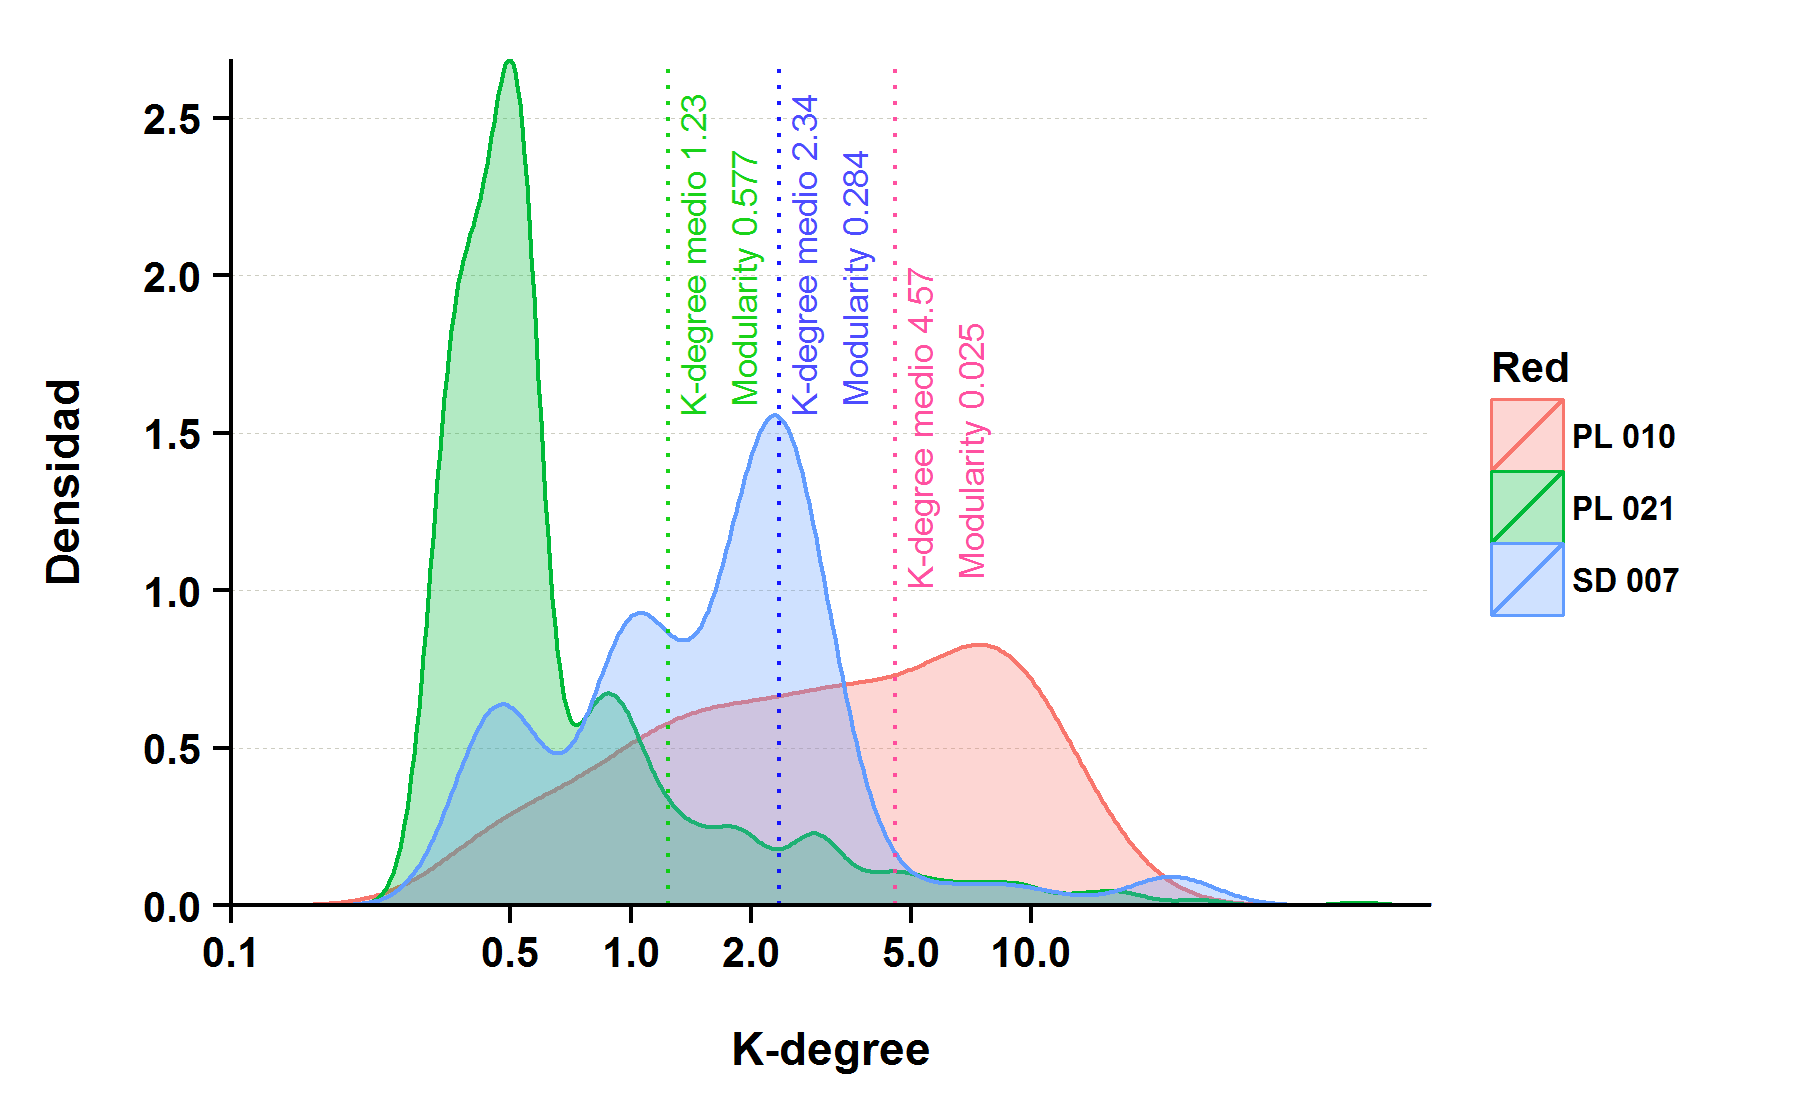
\includegraphics[scale=0.85]{ESTATICA_density_plots.png}
\caption {Distribución de densidad del $k_{degree}$ en tres redes diferentes. Junto a las líneas verticales pueden verse los valores del $\overline {k}_{degree}$ y de la $Modularity$.}
\label{fig:ESTATICA_density_plots}
\end{figure}

Las elevadas correlaciones de $\overline {k}_{radius}$ con $NODF$ y de $\overline {k}_{radius}$ con $Modularity$ son suficientes para esta investigación. Por ejemplo, no se propugna que $log(\overline {k}_{radius})$ sea un buen predictor de $NODF$, de hecho el test de \textit{Shapiro-Wilk} muestra heterocedasticidad. La colección de la \textit{Web of Life} no es una muestra aleatoria, y la distribución de las magnitudes no son normales. Sin embargo, las correlaciones apoyan la idea de que el $\overline {k}_{radius}$ es un indicador global de anidamiento, y el $\overline {k}_{degree}$ de modularidad y que la \textit{descomposición k-core} es una alternativa válida para el estudio del mutualismo.

\subsection{Recableado aleatorio}

Con este experimento se busca entender como se alteran $\overline {k}_{radius}$ y $NODF$ al reconectar al azar un porcentaje de enlaces de la red. La idea subyacente es que las comunidades mutualistas adoptan configuraciones estables, con anidamiento fuerte y $\overline {k}_{radius}$ reducido. Si esto es así, el recableado debe de conducir a un estado más inestable y, eventualmente, a una configuración aleatoria. En el tránsito entre esos dos extremos, la relación encontrada entre las dos magnitudes en el apartado anterior (ecuación \ref{eq:kradius_vs_nodf}) debería de mantenerse. Al reducirse el anidamiento, el $\overline {k}_{radius}$ crecerá de forma lineal.

El experimento comienza recableando al azar un enlace, se analiza la red resultante y se halla la correlación entre $log(\overline {k}_{radius})$  y $NODF$. La operación se repite con $2,3,..,n$ nodos hasta alcanzar un porcentaje fijado de antemano. El experimento se repite $20$ veces para cada red. Se han incluido $50$  redes con más de $40$ enlaces y menos de $200$ para evitar la destrucción abrupta de redes muy pequeñas o un excesivo tiempo de cómputo para las mayores. La figura \ref{fig:ESTATICA_histo_corr_rewiring} es el resultado.

\begin{figure}[h!]
\centering
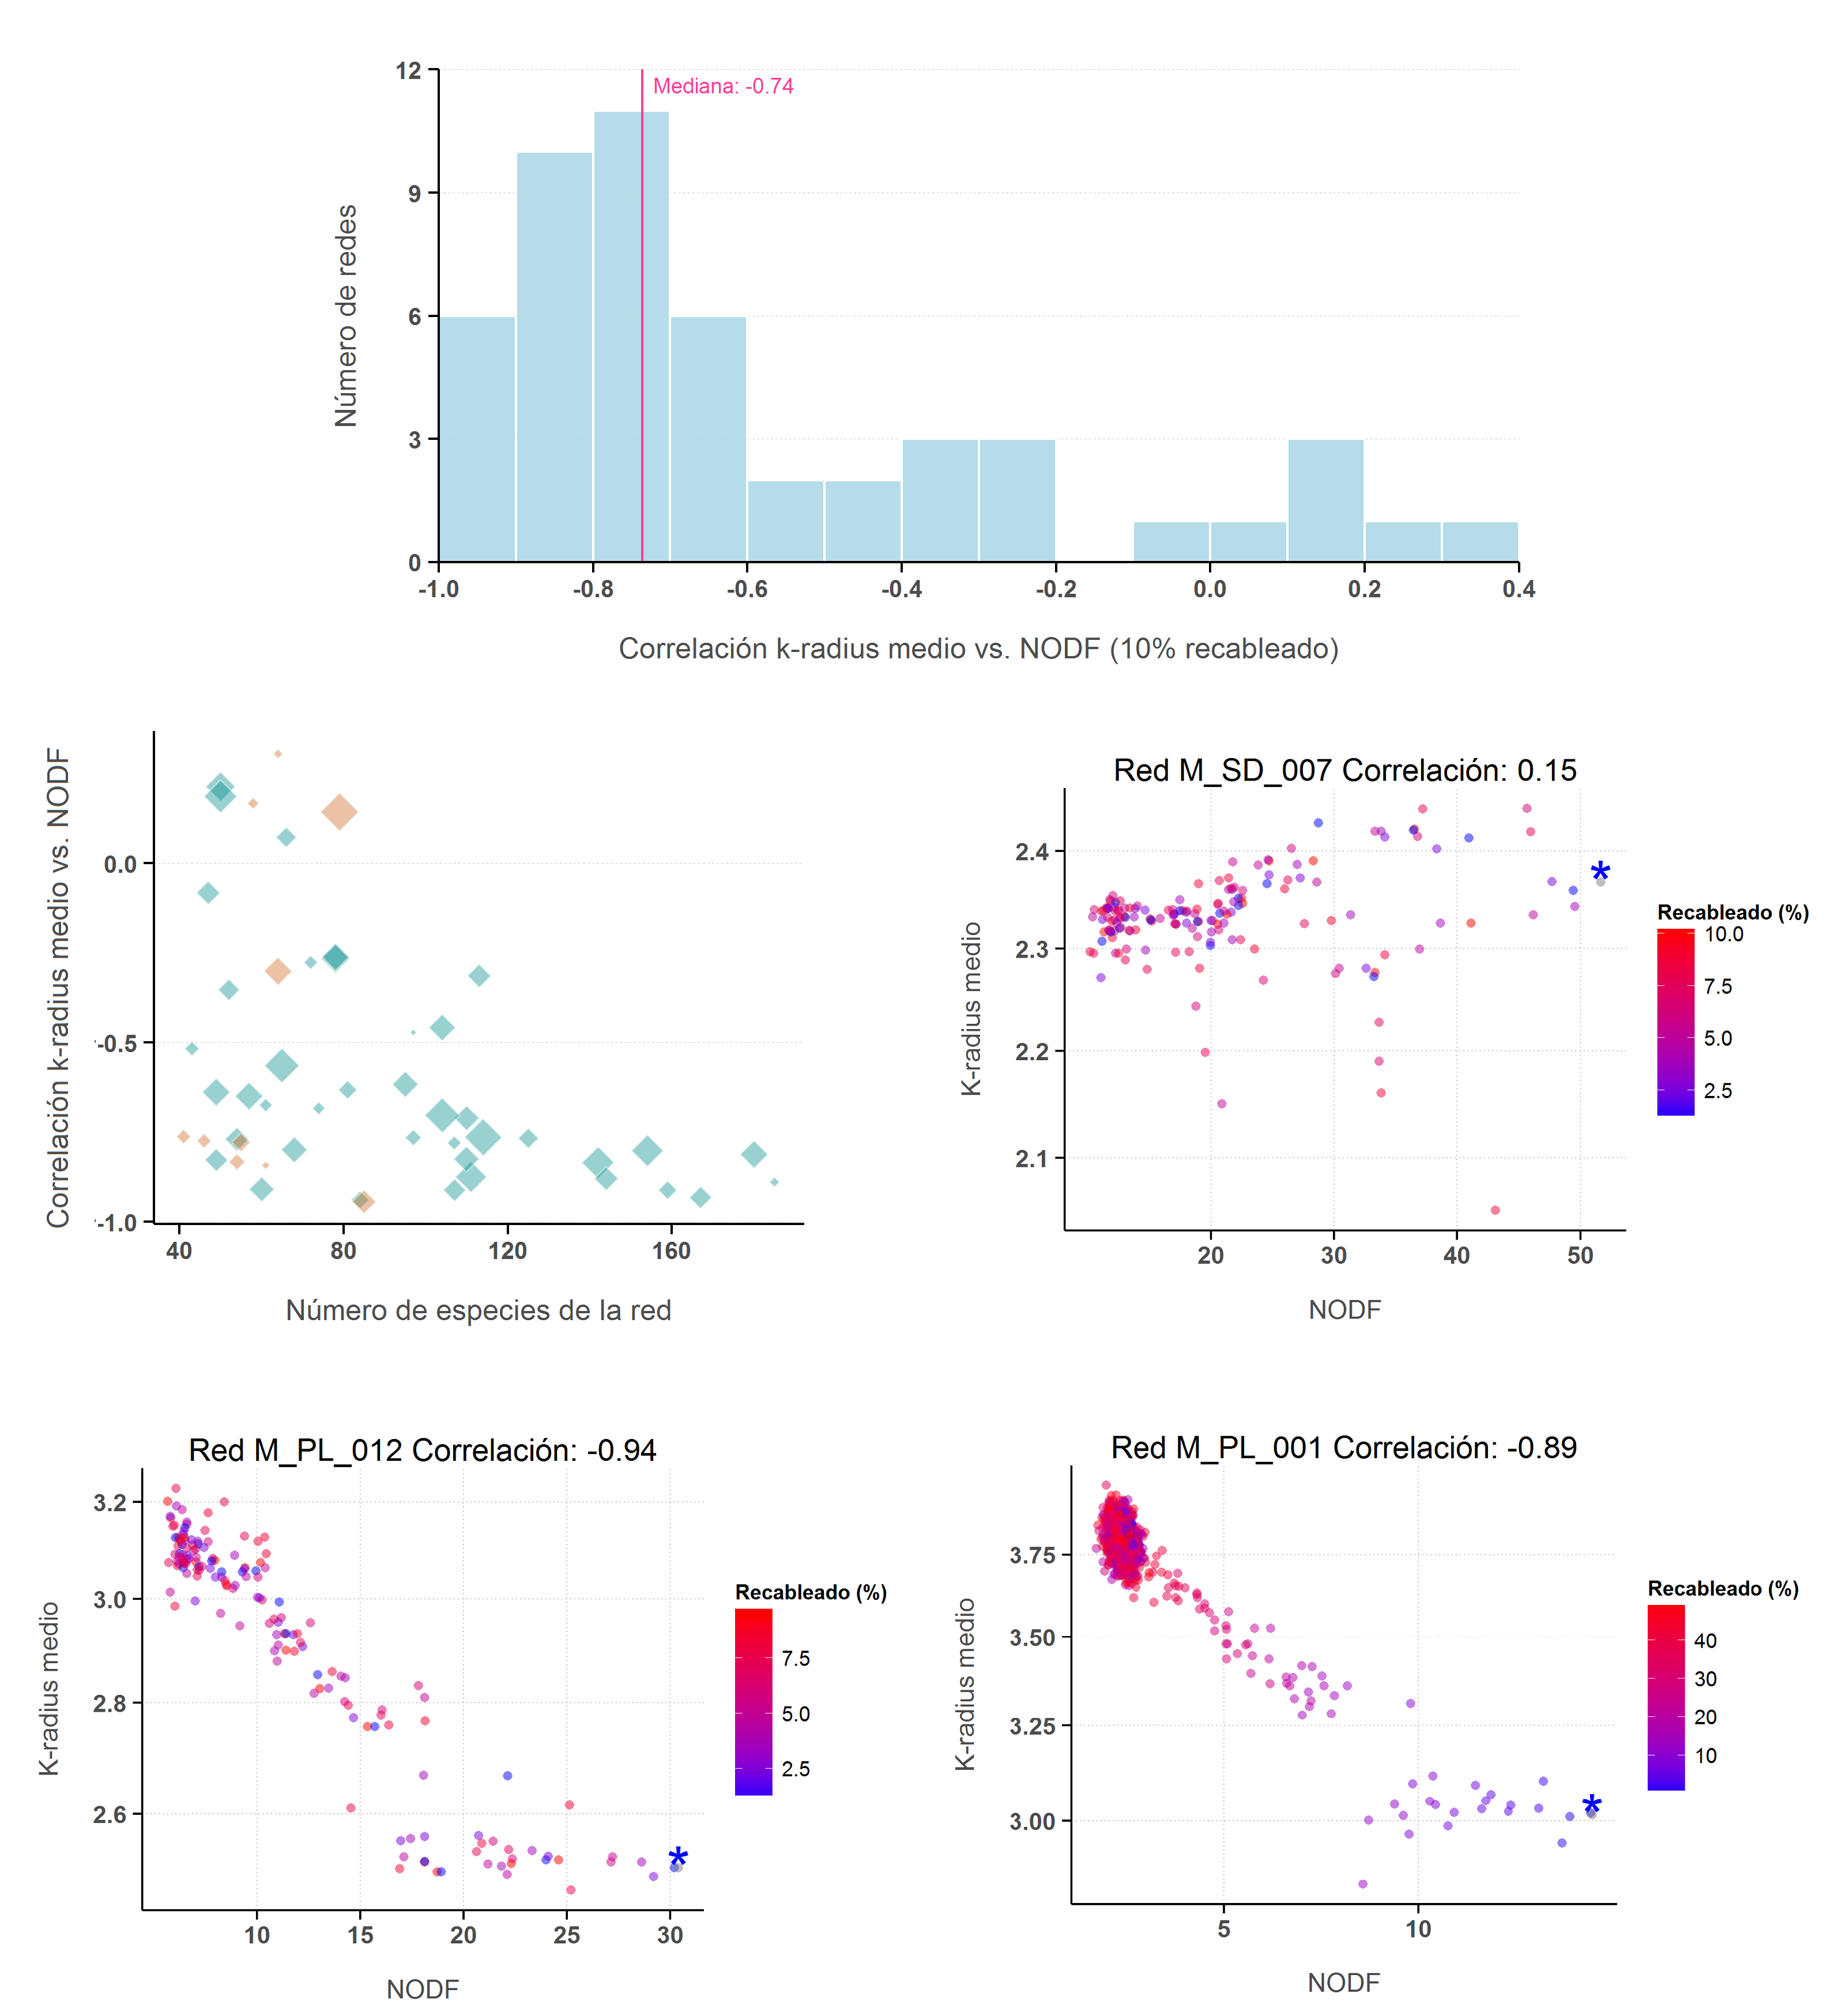
\includegraphics[scale=0.58]{ESTATICA_histo_corr_rewiring.png}
\caption {Resultados del experimento de recableado: histograma de correlación $\overline {k}_{radius}$ y $NODF$, para un máximo del 10\% de enlaces; dispersión en función del tamaño de la red y gráficas para tres redes. En estas últimas el asterico azul indica el valor de la red original, sin modificar ninguna conexión.}
\label{fig:ESTATICA_histo_corr_rewiring}
\end{figure}

El histograma representa los valores de la correlación entre las dos magnitudes aludidas cuando en el experimento se recablean hasta un 10\% de los enlaces. Para la mayoría de las redes se obtienen correlaciones en torno al valor $-0,84$ que se encontró en el apartado anterior. Un pequeño porcentaje de reconexiones hace que $NODF$ se reduzca y que $\overline {k}_{radius}$ aumente de una manera predecible (véase la figura correspondiente a la red $M\_PL\_012$ en la fila inferior). Para las redes que se comportan así, un mayor porcentaje de reconexiones no supone un gran cambio en el estado final. la gráfica de la red $M\_PL\_010$ se ha obtenido cambiando hasta la mitad de los enlaces. Hay una zona de atracción en torno a $\overline {k}_{radius}$ de valor $0,35$ y $NODF$ casi nula, que representa una configuración aleatoria de la red muy alejada de la real.

Hay un porcentaje no despreciable de redes que no siguen esa variación para las que el experimento arroja valores reducidos de correlación e incluso positivos. Es el caso, por ejemplo, de $M\_SD\_007$. Un mínimo cambio destruye el anidamiento sin alterar de manera sustancial el $\overline {k}_{radius}$. Buscando el origen de este comportamiento dispar, se ha representado en la fila intermedia de la figura un diagrama de dispersión que relaciona el valor de la correlación con el número de especies de la red y con la asimetría. Esta se mide como el valor absoluto de la diferencia entre el número de especies de ambas clases dividida por su suma (tabla \ref{table:table_rewiring}) . El área correspondiente al rombo de cada especie es proporcional a esta cantidad. De la gráfica podemos deducir que cuanto mayor es el tamaño de la red, la correlación lineal entre $NODF$ y $log(\overline {k}_{radius})$ tiene mayor tendencia a mantenerse aunque cambie un pequeño porcentaje de conexiones. Para redes más pequeñas, el factor que destruye con mayor rapidez el anidamiento es la asimetría, y la red $M\_SD\_007$ es un caso extremo, con $72$ especies de plantas, solo $7$ de polinizadores y una estructura muy peculiar como se verá en el próximo capítulo de visualizaciones. Estas redes asimétricas son mucho más sensibles a las reconexiones, porque hay una mayor probabilidad de alterar la \textit{k-shell} máxima.

Lo que muestra cualitativamente este experimento, es que cuanto  mayores son el tamaño y la simetría, las redes parecen menos destructibles ante pequeños cambios. El valor de la correlación del experimento de recableado podría utilizarse como indicador numérico de la resistencia a una variación de las condiciones ambientales.

% Table generated by Excel2LaTeX from sheet 'Hoja1'
\begin{table}[ht!]
  \centering
  \tiny
    \begin{tabular}{lrrrr}
    \toprule
    $Red$ & $Plantas$ & $Animales$ & $Asimetría$ & $Correlación \overline r_{radius} y NODF$ \\
    \midrule
    M\_PL\_001 & 84   & 101  & 0,09 & -0,89 \\
    M\_PL\_002 & 43   & 64   & 0,20 & -0,78 \\
    M\_PL\_003 & 36   & 25   & 0,18 & -0,67 \\
    M\_PL\_004 & 12   & 102  & 0,79 & -0,76 \\
    M\_PL\_006 & 17   & 61   & 0,56 & -0,27 \\
    M\_PL\_007 & 16   & 36   & 0,38 & -0,35 \\
    M\_PL\_008 & 11   & 38   & 0,55 & -0,64 \\
    M\_PL\_009 & 24   & 118  & 0,66 & -0,83 \\
    M\_PL\_010 & 31   & 76   & 0,42 & -0,91 \\
    M\_PL\_012 & 29   & 55   & 0,31 & -0,94 \\
    M\_PL\_013 & 9    & 56   & 0,72 & -0,56 \\
    M\_PL\_014 & 29   & 81   & 0,47 & -0,71 \\
    M\_PL\_017 & 25   & 79   & 0,52 & -0,46 \\
    M\_PL\_018 & 39   & 105  & 0,46 & -0,88 \\
    M\_PL\_019 & 40   & 85   & 0,36 & -0,77 \\
    M\_PL\_020 & 20   & 91   & 0,64 & -0,87 \\
    M\_PL\_022 & 21   & 45   & 0,36 & 0,07 \\
    M\_PL\_023 & 23   & 72   & 0,52 & -0,62 \\
    M\_PL\_025 & 13   & 44   & 0,54 & -0,65 \\
    M\_PL\_026 & 105  & 54   & 0,32 & -0,91 \\
    M\_PL\_027 & 18   & 60   & 0,54 & -0,26 \\
    M\_PL\_028 & 41   & 139  & 0,54 & -0,81 \\
    M\_PL\_029 & 49   & 118  & 0,41 & -0,93 \\
    M\_PL\_030 & 28   & 53   & 0,31 & -0,63 \\
    M\_PL\_031 & 48   & 49   & 0,01 & -0,47 \\
    M\_PL\_033 & 13   & 34   & 0,45 & -0,08 \\
    M\_PL\_034 & 26   & 128  & 0,66 & -0,80 \\
    M\_PL\_035 & 61   & 36   & 0,26 & -0,76 \\
    M\_PL\_037 & 10   & 40   & 0,60 & 0,21 \\
    M\_PL\_038 & 8    & 42   & 0,68 & 0,19 \\
    M\_PL\_039 & 17   & 51   & 0,50 & -0,80 \\
    M\_PL\_040 & 29   & 43   & 0,19 & -0,28 \\
    M\_PL\_041 & 31   & 43   & 0,16 & -0,68 \\
    M\_PL\_043 & 28   & 82   & 0,49 & -0,82 \\
    M\_PL\_045 & 17   & 26   & 0,21 & -0,52 \\
    M\_PL\_046 & 16   & 44   & 0,47 & -0,91 \\
    M\_PL\_050 & 14   & 35   & 0,43 & -0,83 \\
    M\_PL\_051 & 14   & 90   & 0,73 & -0,70 \\
    M\_PL\_052 & 15   & 39   & 0,44 & -0,77 \\
    M\_PL\_058 & 32   & 81   & 0,43 & -0,31 \\
    M\_SD\_003 & 25   & 16   & 0,22 & -0,76 \\
    M\_SD\_004 & 34   & 20   & 0,26 & -0,83 \\
    M\_SD\_007 & 72   & 7    & 0,82 & 0,14 \\
    M\_SD\_010 & 50   & 14   & 0,56 & -0,30 \\
    M\_SD\_012 & 35   & 29   & 0,09 & 0,30 \\
    M\_SD\_013 & 36   & 19   & 0,31 & -0,78 \\
    M\_SD\_016 & 24   & 61   & 0,44 & -0,94 \\
    M\_SD\_018 & 29   & 32   & 0,05 & -0,84 \\
    M\_SD\_020 & 25   & 33   & 0,14 & 0,17 \\
    M\_SD\_021 & 18   & 28   & 0,22 & -0,77 \\
    \bottomrule
    \end{tabular}%
  \caption{\label{table:table_rewiring} Resultados del experimento de recableado de hasta un 10\% de enlaces.}
\end{table}%


\subsection{Rendimiento del algoritmo de destrucción}

Como hemos indicado, los resultados de nuestro algoritmo de destrucción se comparan con los obtenidos con \textit{MusRank}, un procedimiento de alto rendimiento. Tras probar diversas posibles combinaciones de los \textit{k-parámetros} encontramos que la más eficiente se basa en ordenar las especies primero por su \textit{k-shell}, a igualdad de  \textit{k-shell} por su $k_{radius}$, y a igualdad de ambos parámetros, por su $k_{degree}$. El área bajo la curva de extinción se utiliza para medir la velocidad de destrucción (mayor cuanto más pequeña). Por ejemplo, la figura \ref{fig:ESTATICA_destruction_comparativa_dosredes} muestra el tamaño de la componente gigante superviviente en función de la fracción de extinciones primarias para la red de polinizadores $M\_PL\_010$ (Elberling \& Olesen, no publicada). A la izquierda, el proceso de destrucción siguiendo el {MusRank}, a la derecha, según la ordenación basada en \textit{k-shell}. Mientras que con \textit{MusRank} la pendiente decreciente permanece casi constante, con \textit{k-shell} puede verse como al eliminarse la \textit{k-shell} máxima se produce una caída abrupta en el número de especies supervivientes.

\begin{figure}[h!]
\centering
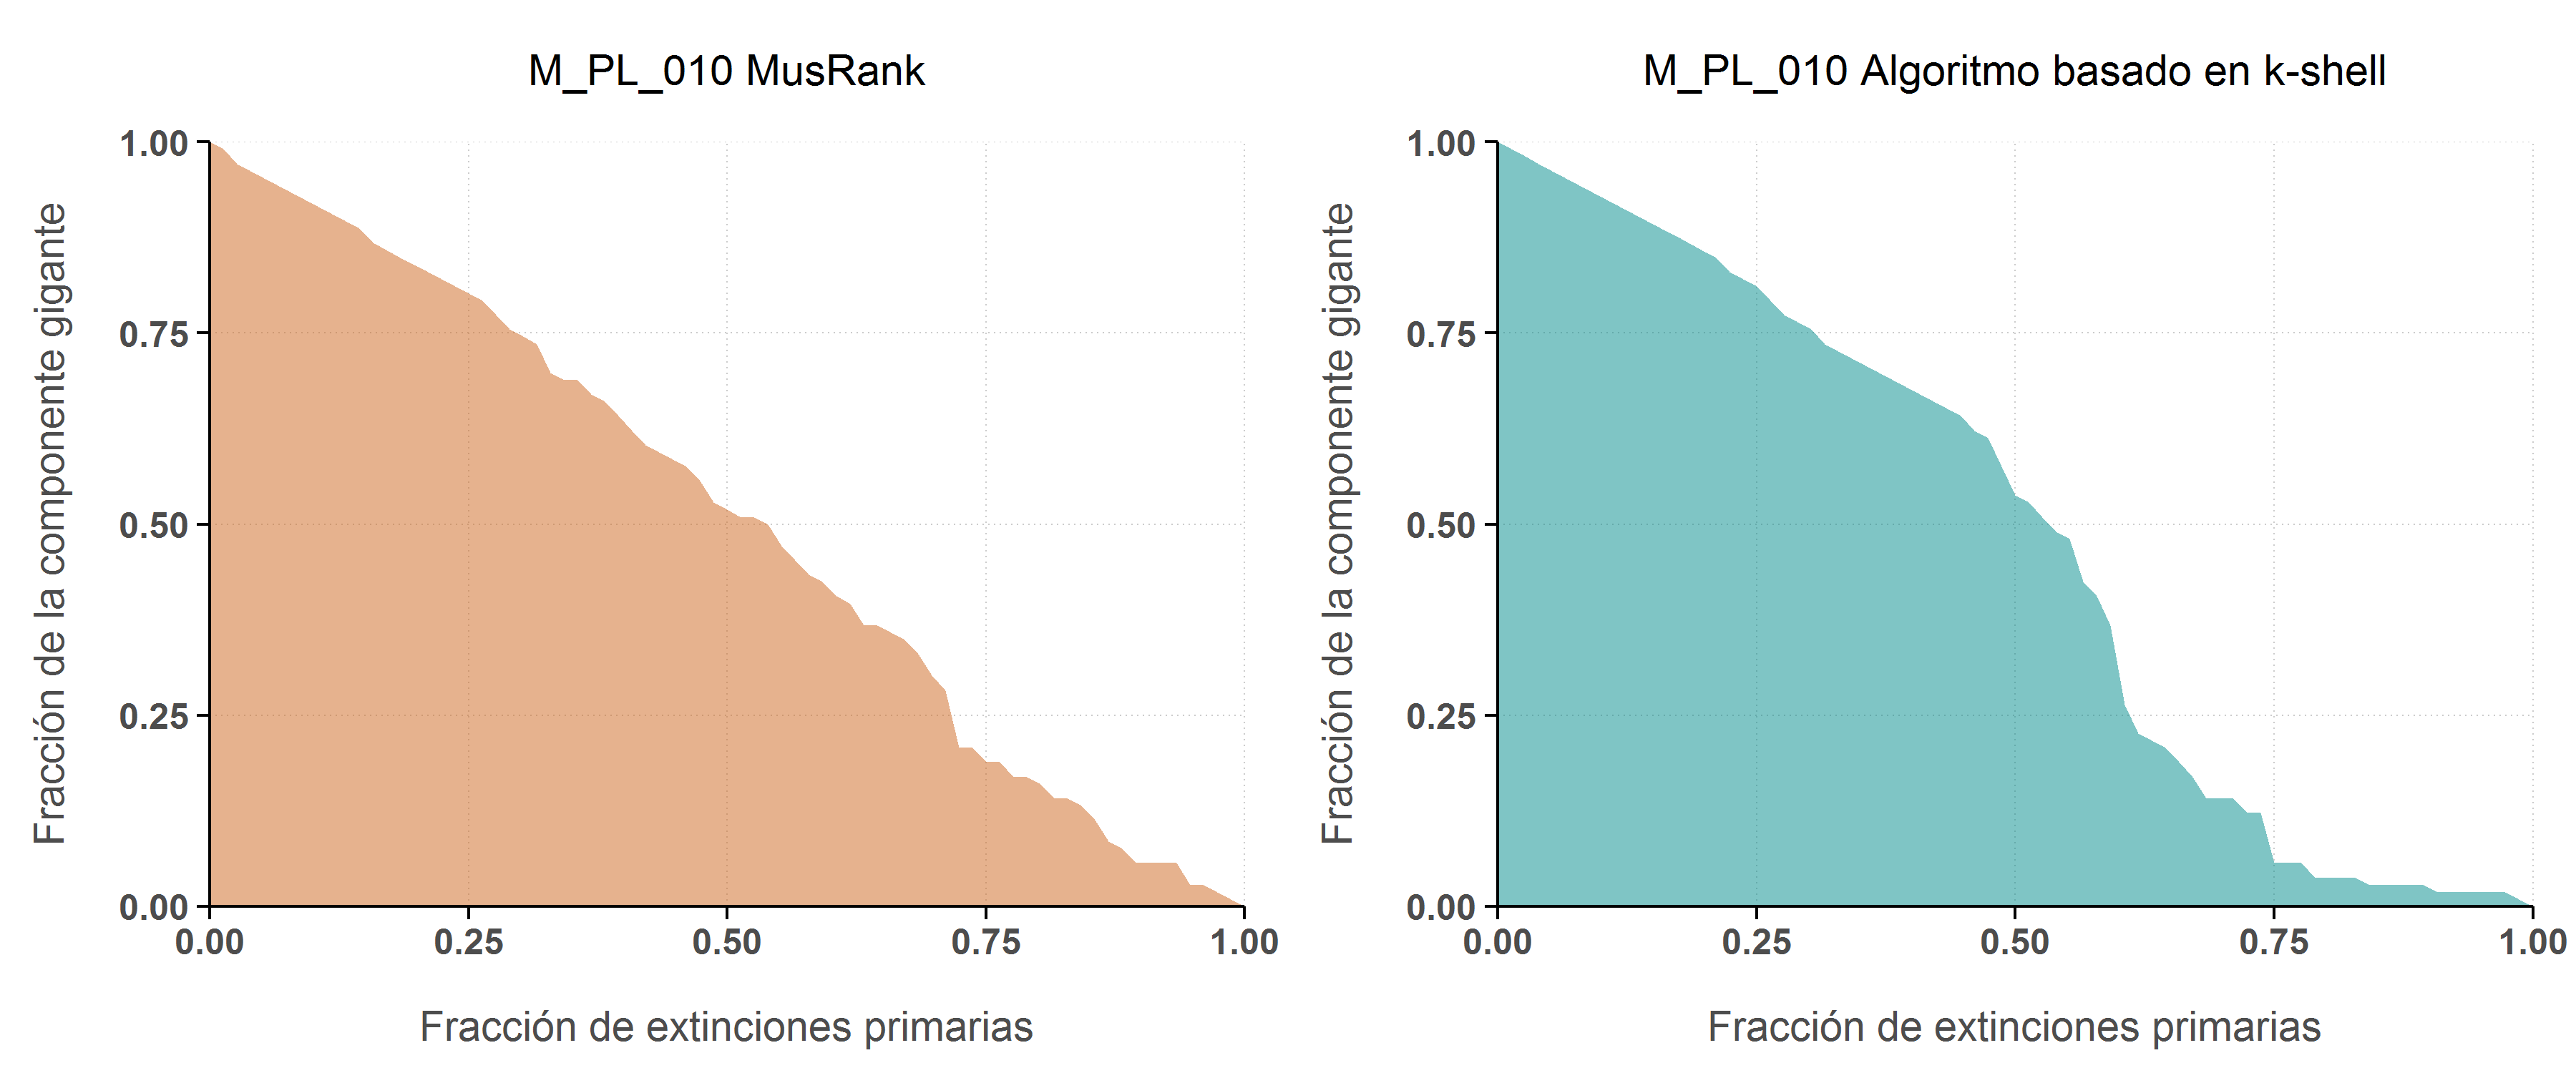
\includegraphics[scale=0.45]{ESTATICA_destruction_comparativa_dosredes.png}
\caption {Curva de extinción de la red planta-polinizador $M\_PL\_010$ para ambos algoritmos}
\label{fig:ESTATICA_destruction_comparativa_dosredes}
\end{figure}

La figura \ref{fig:ESTATICA_destructions_comparison} muestra la comparativa de rendimiento para las $89$ redes del estudio, medida como la diferencia de áreas normalizadas según \textit{MusRank} y según \textit{k-shell}. Si es positiva, el segundo procedimiento es más destructivo y por tanto más eficaz, y viceversa (última columna de la tabla \ref{table:table_results}). la destrucción basada en \textit{k-shell} es más rápida para $57$ de las $59$ redes del tipo \textit{planta-polinizador}. 

\begin{figure}[h!]
\centering
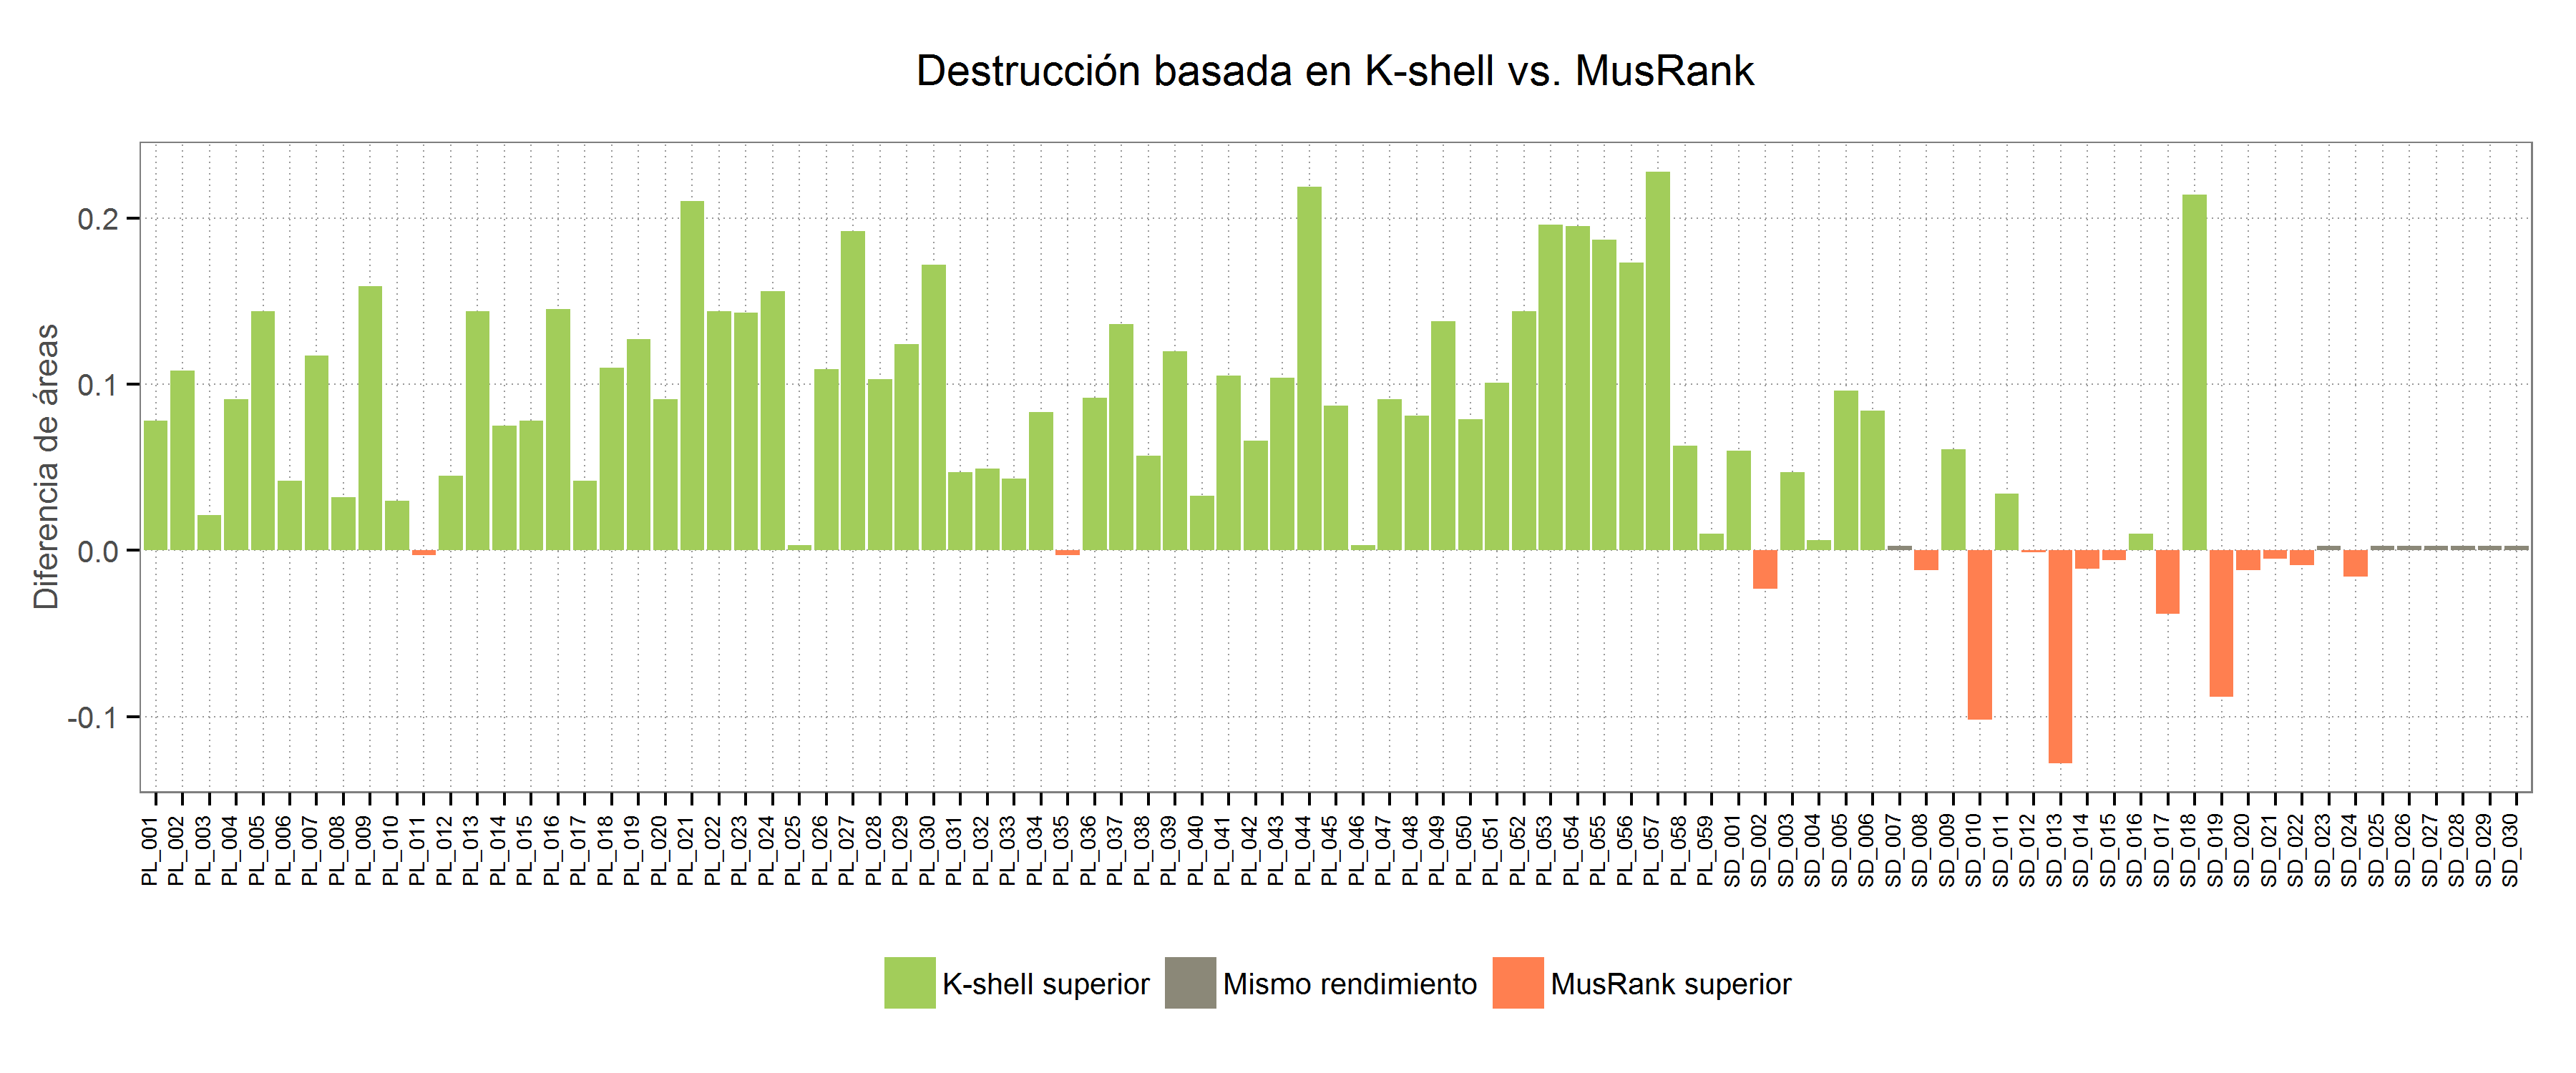
\includegraphics[scale=0.5]{ESTATICA_destructions_comparison.png}
\caption {Comparison of destruction performance of \textit{k-shell} ranking based algorithm vs. \textit{MusRank}}
\label{fig:ESTATICA_destructions_comparison}
\end{figure}

La diferencia de rendimiento no es tan llamativa para las de dispersores de semillas, \textit{MusRank} supera a \textit{k-shell} en $13$ casos, es más lento en $10$ y equivalente en $y$. Como hemos visto, las redes de este tipo en la colección estudiada son de menor tamaño y más anidades. El procedimiento basado en \textit{k-shell} parece ser mejor predictor de la resistencia de la red en comunidades grandes y modulares, mientras que \textit{MusRank} alcanza mejor rendimiento para redes pequeñas y fuertemente anidadas.

\section{Conclusiones}

La \textit{descomposición k-core} proporciona una sólida base para el análisis del mutualismo. Hemos demostrado como las \textit{k-magnitudes} definidas como propiedades surgidas del procedimiento, permiten conocer en detalle la estructura de las redes. En particular, al promediar los valores locales para todo el sistema, $\overline {k}_{radius}$ y $\overline {k}_{degree}$ muestran una fuerte correlación con los observables globales $NODF$ y $Modularity$. 

Esta técnica descubre detalles internos de una forma natural, agrupando las especies en conjuntos que comparten propiedades topológicas. La identificación de las distintas \textit{k-shells} permite realizar estudios de estabilidad y resistencia. La simulación de perturbaciones externas puede concentrarse en la destrucción de las \textit{k-shells} más internas y observar el efecto para la supervivencia de la comunidad. 

La descomposición es también el criterio de una nueva ordenación de las especies. Hemos provocado extinciones primarias y evaluado la evolución del tamaño de la componente gigante. Los resultados muestra que el procedimiento de extinción basado en \textit{k-shell} obtiene un mejor renidmiento que \textit{MusRank} para casi todas las redes de polinizadores de la colección investigada, y es ligeramente peor para las de dispersores de semillas. La ordenación por \textit{k-core} es un buen predictor de la resistencia de red.

Aunque hemos enfocado el estudio en redes mutualistas, la técnica se puede extender a otros tipos de redes bipartitas, por ejemplo comensalistas. Relaciones bipartitas y con fuerte anidamiento, como las que aparecen en redes de innovación y comercio, podrían también beneficiarse de este análisis.